\documentclass[11pt]{article}

\usepackage[margin=0.65in]{geometry}
\usepackage[T1]{fontenc}
\usepackage[utf8]{inputenc}
\usepackage{lmodern}
\usepackage{array}
\usepackage{booktabs}
\usepackage{longtable}
\usepackage{tabularx}
\usepackage{caption}
\usepackage{float}
\usepackage{graphicx}
\usepackage{hyperref}
\usepackage{parskip}
\usepackage{ragged2e}
\usepackage{setspace}
\usepackage{enumitem}
\usepackage{needspace}
\usepackage[table]{xcolor}
\usepackage{tikz}
\usepackage{fancyhdr}
\usepackage{transparent}

\usetikzlibrary{arrows.meta,positioning,fit,calc}
\usepackage[natbibapa]{apacite}

\definecolor{PrimaryRed}{HTML}{8B1E1E}
\definecolor{DeepNavy}{HTML}{15324A}
\definecolor{MidTeal}{HTML}{287D7A}
\definecolor{SoftBlue}{HTML}{DDEEFF}
\definecolor{SoftGreen}{HTML}{E4F1E8}
\definecolor{SoftGold}{HTML}{F8EDC7}
\definecolor{SoftRose}{HTML}{F5E2E7}
\definecolor{SoftGray}{HTML}{F4F4F4}

\definecolor{AccessBlue}{HTML}{4F7FA8}
\definecolor{MeaningGold}{HTML}{A67C22}
\definecolor{RoutesGreen}{HTML}{4F7D60}
\definecolor{ActionRose}{HTML}{A85C70}

\definecolor{MapAccess}{HTML}{DDEEE7}
\definecolor{MapEvidence}{HTML}{F4E1E6}
\definecolor{MapRoutes}{HTML}{E0E9F6}
\definecolor{MapAction}{HTML}{E7F0D6}

\newcommand{\tocmark}[1]{%
  \textcolor{#1}{\rule{0.09in}{0.09in}}\hspace{0.07in}%
}

\hypersetup{
  colorlinks=true,
  linkcolor=DeepNavy,
  urlcolor=DeepNavy,
  citecolor=DeepNavy,
  pdftitle={Communication as Access-to-Agency},
  pdfauthor={Piter Zacari Garcia Bautista},
  pdfsubject={EDE 448 Communication and Positive Behavioral Support Strategies and Resources Portfolio},
  pdfkeywords={communication, AAC, sensory access, positive behavior support, inclusion, Puzzle Plan, EQUITAS}
}

\setlength{\parindent}{0pt}
\setstretch{1.045}
\setlist[itemize]{leftmargin=0.22in,itemsep=0.025in,topsep=0.04in}
\setlist[enumerate]{leftmargin=0.25in,itemsep=0.025in,topsep=0.04in}
\captionsetup{font=small,labelfont=bf,labelsep=period}
\bibliographystyle{apacite}
\setlength{\headheight}{22pt}

\pagestyle{fancy}
\fancyhf{}
\fancyhead[L]{\small\color{DeepNavy}Communication as Access-to-Agency}
\fancyhead[R]{\small\color{DeepNavy}EDE 448 Portfolio}
\fancyfoot[C]{\small\thepage}
\renewcommand{\headrulewidth}{0.4pt}
\renewcommand{\headrule}{\hbox to\headwidth{\color{PrimaryRed}\leaders\hrule height \headrulewidth\hfill}}

\newcommand{\toolsection}[1]{%
  \Needspace{4\baselineskip}
  \vspace{0.065in}\noindent{\normalsize\bfseries\color{PrimaryRed}#1}
  \par\vspace{0.02in}
}

\newcommand{\resourceheading}[5]{%
  \clearpage
  \phantomsection

    \ifnum#1<4
  \addcontentsline{toc}{section}{\protect\tocmark{AccessBlue}Resource #1: #2}
\else
  \ifnum#1<6
    \addcontentsline{toc}{section}{\protect\tocmark{MeaningGold}Resource #1: #2}
  \else
    \ifnum#1=6
      \addcontentsline{toc}{section}{\protect\tocmark{RoutesGreen}Resource #1: #2}
    \else
      \ifnum#1=7
        \addcontentsline{toc}{section}{\protect\tocmark{ActionRose}Resource #1: #2}
      \else
        \ifnum#1=8
          \addcontentsline{toc}{section}{\protect\tocmark{RoutesGreen}Resource #1: #2}
        \else
          \ifnum#1=9
            \addcontentsline{toc}{section}{\protect\tocmark{ActionRose}Resource #1: #2}
          \else
            \addcontentsline{toc}{section}{\protect\tocmark{RoutesGreen}Resource #1: #2}
          \fi
        \fi
      \fi
    \fi
  \fi
\fi
  
  {\color{PrimaryRed}\rule{\textwidth}{1.2pt}}\par
  \vspace{0.08in}
  {\Large\bfseries\color{DeepNavy}Resource #1: #2}\par
  \vspace{0.07in}
  \colorbox{SoftBlue}{%
    \parbox{\dimexpr\textwidth-2\fboxsep\relax}{%
      \small
      \textbf{Area:} #3\hfill\textbf{Primary audience:} #4\\
      \textbf{Practice origin:} #5
    }%
  }
  \vspace{0.08in}
}

\newcommand{\reflectionbox}[1]{%
  \vspace{0.06in}
  \noindent\colorbox{SoftGold}{%
    \parbox{\dimexpr\textwidth-2\fboxsep\relax}{%
      \small\textbf{Evidence and reflection.} #1
    }%
  }
  \vspace{0.05in}
}

\newcommand{\adaptationbox}[1]{%
  \vspace{0.06in}
  \noindent\colorbox{SoftGreen}{%
    \parbox{\dimexpr\textwidth-2\fboxsep\relax}{%
      \small\textbf{Adaptation and limitation.} #1
    }%
  }
  \vspace{0.05in}
}

\newcommand{\sourcebox}[1]{%
  \vspace{0.06in}
  \noindent{\small\color{DeepNavy}\textbf{Key sources and links.} #1}
}

\newcommand{\restrictedartifact}[2]{%
  \IfFileExists{#1}{%
    \includegraphics[width=#2]{#1}%
  }{%
    \fcolorbox{DeepNavy}{SoftGray}{%
      \parbox{0.86\textwidth}{%
        \centering\small\vspace{0.15in}
        \textbf{Restricted artifact image omitted from this public course-repository checkout.}\\[0.03in]
        The completed page is included only in the authorized Warner School submission package.
        \vspace{0.15in}
      }%
    }%
  }%
}

\newcommand{\restrictedartifactpanel}[4]{%
  \begingroup
  \begin{minipage}[c][#3][c]{#2}
    \centering
    \IfFileExists{#1}{%
      \includegraphics[width=\linewidth,height=#3,keepaspectratio]{#1}%
    }{%
      \setlength{\fboxsep}{4pt}%
      \fcolorbox{DeepNavy}{SoftGray}{%
        \parbox[c][\dimexpr#3-2\fboxsep-2\fboxrule\relax][c]{\dimexpr\linewidth-2\fboxsep-2\fboxrule\relax}{%
          \centering\scriptsize
          \textbf{Restricted visual omitted from the public course-repository build.}\\[0.02in]
          #4
        }%
      }%
    }%
  \end{minipage}%
  \endgroup
}

\newcommand{\tableheaderthree}[3]{%
  \rowcolor{PrimaryRed}
  \color{white}\bfseries #1 &
  \color{white}\bfseries #2 &
  \color{white}\bfseries #3 \\
}

\newcommand{\tableheaderfour}[4]{%
  \rowcolor{PrimaryRed}
  \color{white}\bfseries #1 &
  \color{white}\bfseries #2 &
  \color{white}\bfseries #3 &
  \color{white}\bfseries #4 \\
}

\begin{document}

\hypersetup{pageanchor=false}
\begin{titlepage}
\newgeometry{margin=0.72in}
\thispagestyle{empty}

\begin{center}
{\large University of Rochester\\}
{\normalsize Warner School of Education\\[0.16in]}

{\color{PrimaryRed}\rule{\textwidth}{1.5pt}}\\[0.16in]
{\Huge\bfseries Communication as\\[0.06in]Access-to-Agency \& Empowerment}\\[0.16in]
{\LARGE Communication and Positive Behavioral\\[0.04in]Support Strategies and Resources Portfolio}\\[0.13in]
{\large EDE 448 --- Summer 2026}\\[0.10in]

\vfill

\begin{tikzpicture}[
  node distance=0.18in,
  pillar/.style={draw=DeepNavy, rounded corners=2pt, minimum width=1.42in,
    minimum height=0.76in, align=center, font=\scriptsize\bfseries, inner sep=4pt},
  flow/.style={-{Latex[length=2.0mm]}, line width=0.8pt, draw=PrimaryRed}
]
\node[pillar, fill=SoftBlue] (memo) {30-SECOND\\VIDEO MEMO};
\node[pillar, fill=SoftGold, right=of memo] (souvenir) {EVERY-DAY\\SOUVENIR};
\node[pillar, fill=SoftGreen, right=of souvenir] (recap) {DAILY RECAP\\EVIDENCE STORY};
\node[pillar, fill=SoftRose, right=of recap] (family) {WEEKLY RECAP \&\\ FAMILY SHARED STORY};
\draw[flow] (memo) -- (souvenir);
\draw[flow] (souvenir) -- (recap);
\draw[flow] (recap) -- (family);
\end{tikzpicture}

\vfill

\colorbox{SoftBlue}{%
\parbox{0.90\textwidth}{%
\centering\small\vspace{0.02in}
\textbf{Ten practical resources for teachers, families, and support teams}\\[0.04in]
Implemented camp artifacts anchor the collection; connected course tools extended the same commitments to sensory access, PTR, AAC, peer participation, and classroom practice.
}%
}
\end{center}

\vfill

\begin{center}
\renewcommand{\arraystretch}{1.18}
\setlength{\tabcolsep}{4pt}
\begin{tabular}{>{\bfseries\raggedleft\arraybackslash}p{1.90in} >{\raggedright\arraybackslash}p{5.08in}}
Student & Piter Zacari Garcia Bautista \\
Course & Communication and Positive Behavioral Supports (CPBS) for Students with Autism and Other Complex Needs (EDE 448)\\
Assignment & CPBS Strategies and Resources Portfolio \\
Professional Context & Inclusive, tech-rich upper-elementary \& middle school learning environments \\
Interpretive Framework & Puzzle Plan, with EQUITAS at its equity-centered heart \\
Due Date & August 7, 2026 \\
\end{tabular}
\end{center}

\vfill

\begin{center}
\begin{minipage}{0.94\textwidth}
\small

My teaching placement taught me to make participation routes visible and to treat student action, questions, artifacts, and multimodal responses as evidence. The \textsc{Puzzle Plan} carried that learning into camp as an interdisciplinary framework connecting lived experience, education, data, and research so that no single diagnosis, behavior, observation, or score becomes the whole learner. \textsc{EQUITAS}, its equity-centered heart, asks whose knowledge is included, what context is missing, how power and bias shape interpretation, and whether a decision expands access, dignity, agency, and belonging. Across this portfolio, those questions test not only whether behavior changes, but whether learners gain meaningful influence over the goal, method, communication route, interpretation, and definition of success.
\end{minipage}


\vspace{0.12in}
\fcolorbox{PrimaryRed}{SoftRose}{%
\parbox{0.90\textwidth}{%
\centering\small
\textbf{Restricted Educational Use Notice}\\[0.03in]
\textit{Not for public or external distribution.} This portfolio is provided solely for course-related teaching, learning, assessment, and internal review within the University of Rochester Warner School of Education.
}%
}
\end{center}

\restoregeometry
\end{titlepage}
\hypersetup{pageanchor=true}
\pagenumbering{roman}

% \section*{Assignment and Design Standard}
% \addcontentsline{toc}{section}{Assignment and Design Standard}

% This culminating portfolio is worth 40 percent of the EDE448 grade and is due August 7, 2026. The Blackboard prompt contains the internally inconsistent phrase ``at least ten (8) resources/supports.'' I use the more demanding interpretation: ten resources, each designed to stand alone within one or two pages. Every entry explains the support for a teacher or family audience, connects it to communication, social-emotional learning, or behavior, identifies when and why it should be used, and provides relevant sources or websites. The ten resources occupy 20 pages; the title, assignment standard, contents, portfolio map, closing reflection, and references are six framing pages and are not counted toward the resource limit. The complete PDF therefore contains 26 physical pages.

% The portfolio reworks applicable Module 1, 2, and 3 assignments into practitioner tools rather than stacking ten old papers together. Its evidence core is a communication system already built through EDU486: a 30-second student video memo after an activity, an every-day personalized souvenir, a day recap evidence story, and a full-week personalized family recap organized per attended day and per activity. Six connected EDE448 resources extend the same commitments to sensory access, peer culture, PTR, AAC, backup communication, and flexible roles. Six artifact visuals are reproduced under signed parent/guardian consent for this internal UofR educational review; family contacts, private correspondence, and unrelated records are not reproduced.

% \toolsection{How the Rubric Is Made Visible}

% \renewcommand{\arraystretch}{1.17}
% \setlength{\tabcolsep}{5pt}
% \begin{tabularx}{\textwidth}{>{\bfseries\RaggedRight\arraybackslash}p{1.70in} >{\RaggedRight\arraybackslash}X}
% \rowcolor{PrimaryRed}
% \color{white}Rubric Area & \color{white}Portfolio Evidence \\
% Scholarly connections & Claims are cited at the point of use and linked to instructional decisions; the reference list uses APA-style source information. \\
% \rowcolor{SoftGray}
% Organization and clarity & Ten numbered, categorized resources follow one repeated structure and include ready-to-use tables, scripts, checklists, or visuals. \\
% Relevance to practice & Every resource names a setting, implementation sequence, evidence to notice, and concrete teacher/family actions. \\
% \rowcolor{SoftGray}
% Evidence and reflection & Each entry distinguishes observation from inference, names limitations, and identifies conditions that would trigger adaptation. \\
% \end{tabularx}

% \toolsection{Evidence Boundary}

% The Pine Brook technology-placement examples remain de-identified practice records, not diagnoses or universal student traits. The contents page and Resources 4, 5, 7, and 9 reproduce completed EDU486 visuals, including participant names and photographs, under signed parent/guardian consent for this internal UofR educational submission. Plans do not prove implementation; photographs show action but not complete understanding; automatic transcripts require source review before direct quotation. Day 5 has photographs and a same-session clean transcript but no source video. The full-week family packages were completed and prepared for delivery, but no delivery receipt or family response was recovered. The Communication Support Plan remains prospective and never claims that a particular camper used AAC; the Kit for Kids evidence remains limited to de-identified teacher notes and two anonymous responses.

\clearpage

\vfill
\begin{center}
{\normalsize\bfseries\color{DeepNavy}How the Resources Move Evidence Toward Agency}\par
\vspace{0.08in}

\begin{tikzpicture}[
  stage/.style={draw=DeepNavy, rounded corners=2pt, minimum width=1.48in,
    minimum height=0.78in, align=center, font=\scriptsize, inner sep=5pt},
  route/.style={-{Latex[length=1.8mm]}, line width=0.75pt, draw=PrimaryRed}
]

\node[stage, fill=SoftBlue] (notice) {
  \textbf{NOTICE ACCESS}\\
  sensory access, peer inclusion,\\
  PTR support\\
  \textit{Resources 1--3}
};

\node[stage, fill=SoftGold, right=0.16in of notice] (record) {
  \textbf{RECORD MEANING}\\
  video memo and personalized\\
  science souvenir\\
  \textit{Resources 4--5}
};

\node[stage, fill=SoftGreen, right=0.16in of record] (keep) {
  \textbf{KEEP ROUTES OPEN}\\
  AAC, low-tech backup,\\
  flexible peer roles\\
  \textit{Resources 6, 8, 10}
};

\node[stage, fill=SoftRose, right=0.16in of keep] (return) {
  \textbf{RETURN FOR ACTION}\\
  day recap and full-week\\
  family recap\\
  \textit{Resources 7, 9}
};

\draw[route] (notice) -- (record);
\draw[route] (record) -- (keep);
\draw[route] (keep) -- (return);

\node[
  draw=MidTeal,
  fill=white,
  rounded corners=2pt,
  below=0.17in of $(record.south)!0.5!(keep.south)$,
  minimum width=3.20in,
  minimum height=0.38in,
  align=center,
  font=\scriptsize
] {
  \textbf{Puzzle Plan + EQUITAS:}
  whose evidence survives, and what does it change?
};

\end{tikzpicture}

\vspace{0.07in}

\parbox{0.86\textwidth}{\centering\small
Read the collection as a connected path: examine access conditions, preserve student meaning and evidence, keep communication and participation routes open, and return that evidence toward planning, family partnership, and meaningful action.}

\end{center}

\vfill
\tableofcontents
\vfill



\clearpage
\pagenumbering{arabic}

\vfill
% \small
\setlength{\tabcolsep}{4pt}

\arrayrulecolor{DeepNavy!20}
\setlength{\arrayrulewidth}{0.75pt}

\begin{longtable}{
  >{\centering\arraybackslash}p{0.1in}
  >{\RaggedRight\arraybackslash}p{2.40in}
  >{\RaggedRight\arraybackslash}p{1.80in}
  >{\RaggedRight\arraybackslash}p{2.50in}
}

\rowcolor{DeepNavy}
\color{white}\bfseries \# &
\color{white}\bfseries Resource &
\color{white}\bfseries Primary Area &
\color{white}\bfseries Assignment/Evidence Origin \\

\rowcolor{MapAccess}
1 & Sensory Access Walk and Redesign Checklist & Sensory/environment & Module 1 Sensory Walk; Pine Brook placement \\
\hline

\rowcolor{MapAccess}
2 & Many Ways to Be a Good Classmate & Inclusion/SEL & Module 1 taught Kit for Kids lesson; placement \\
\hline

\rowcolor{MapAccess}
3 & PTR Evidence-to-Support Planning Guide & Positive behavior support & Module 2 PTR assignment; placement event \\
\hline

\rowcolor{MapEvidence}
4 & 30-Second Student Video Memo & Student voice/formative support & Implemented post-activity memos; de-identified transcript records \\
\hline

\rowcolor{MapEvidence}
5 & Every-Day Personalized Science Souvenir & Recognition/continuity & Implemented personalized souvenirs; activity evidence \\
\hline

\rowcolor{MapRoutes}
6 & AAC Tool Selection and Implementation Guide & AAC & Module 3 TD Snap review; Grade 2 curriculum \\
\hline

\rowcolor{MapAction}
7 & Day Recap Evidence Story & Collective memory/planning & Five implemented and reviewed recap decks \\
\hline

\rowcolor{MapRoutes}
8 & Low-Tech AAC Backup Starter & AAC continuity & Module 3 system; camp sensory feedback \\
\hline

\rowcolor{MapAction}
9 & Full-Week Personalized Family Recap & Family partnership & Module 3 logs; completed day-by-day family recap books \\\hline

\rowcolor{MapRoutes}
10 & Flexible Peer Roles and Participation Routes & Social interaction & Kit lesson; Identity Beads; policy/showcase roles \\\hline

\end{longtable}
\normalsize


\vfill
\begin{center}

\transparent{0.85}{
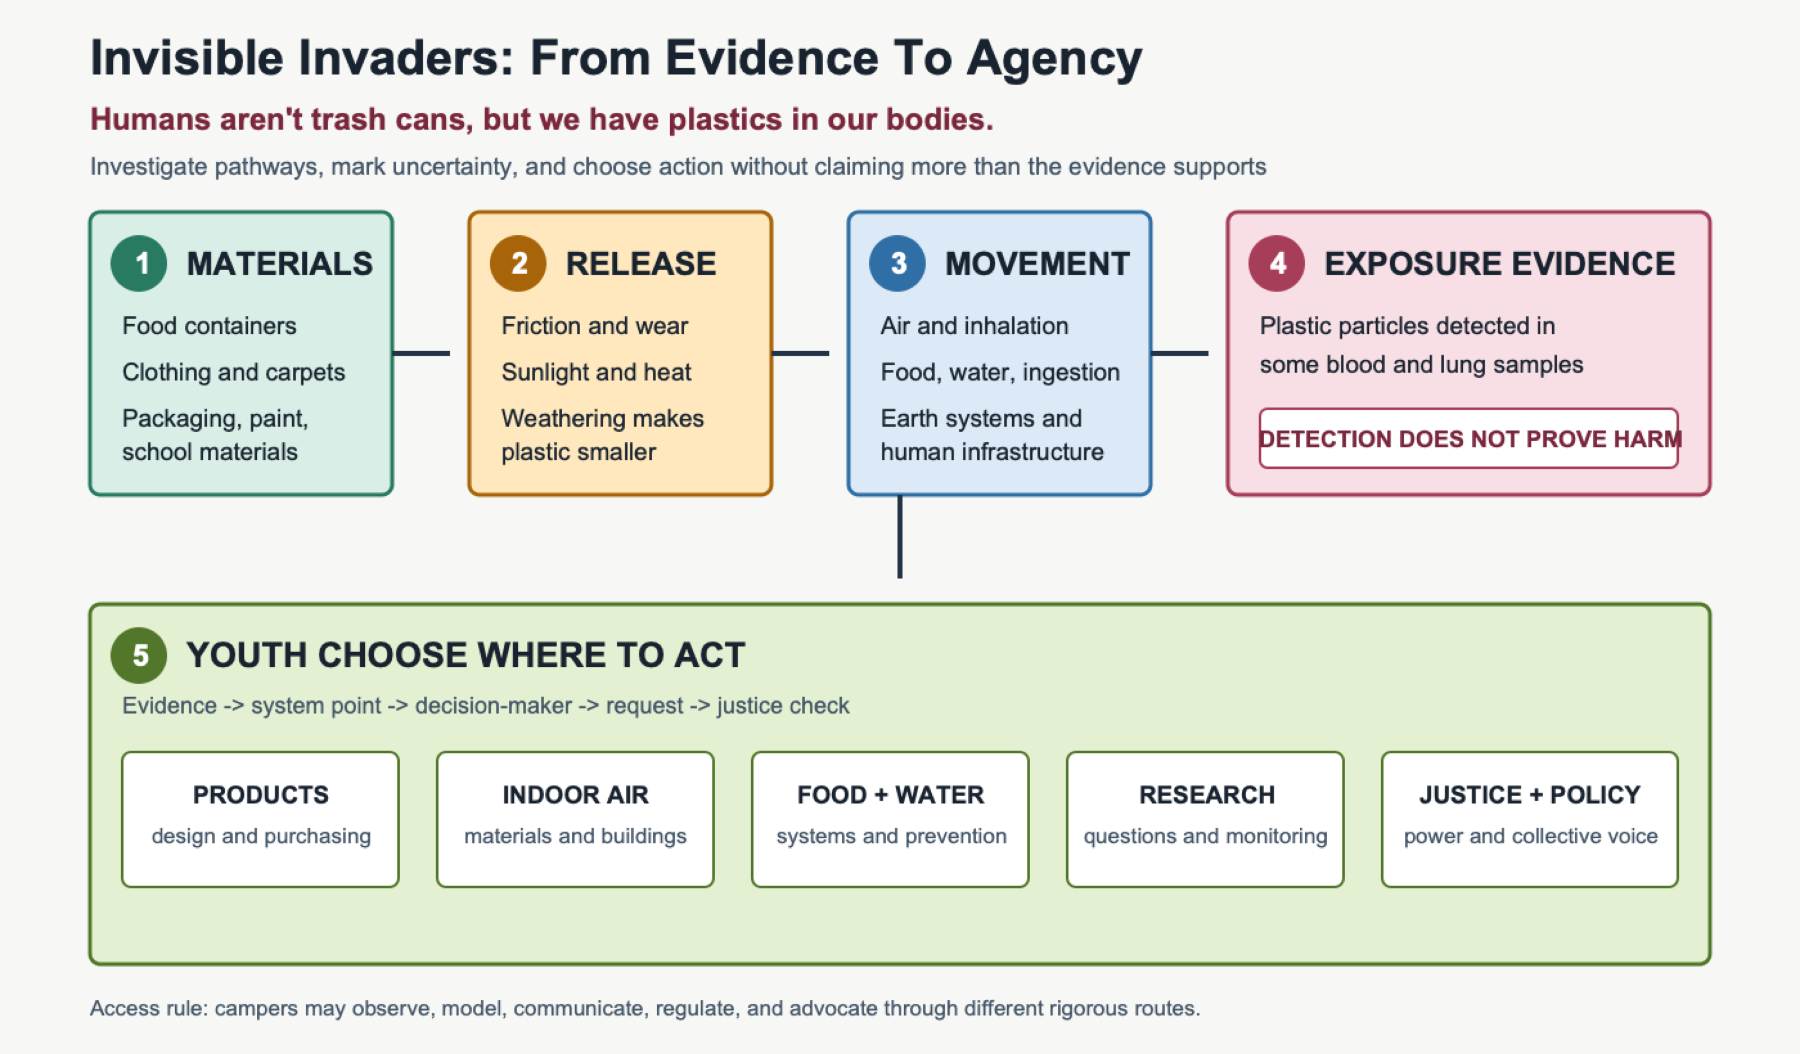
\includegraphics[
  width=0.9\textwidth,
  keepaspectratio
]{assets/artifact-previews/Invisible Invaders - Evidence to Agency Pathway.png}
}

% \vspace{0.08in}
{\small\color{DeepNavy}
\textbf{Portfolio design map.}
\textit{Invisible Invaders} brings the portfolio's central commitments together: evidence, access, multimodal participation, communication, regulation, and youth agency move through a connected system toward meaningful action.}

\end{center}
\vfill


% \vspace{0.05in}
% \begin{center}
% {\normalsize\bfseries\color{DeepNavy}Reusable Camp Access Board}\par
% \vspace{0.06in}
% \begin{tikzpicture}[
%   route/.style={draw=MidTeal, rounded corners=1.5pt, minimum width=1.30in,
%     minimum height=0.40in, align=center, font=\scriptsize\bfseries, inner sep=3pt}
% ]
% \node[route, fill=SoftBlue] (talk) {TALK};
% \node[route, fill=SoftGold, right=0.10in of talk] (point) {POINT};
% \node[route, fill=SoftGreen, right=0.10in of point] (draw) {DRAW / WRITE};
% \node[route, fill=SoftRose, right=0.10in of draw] (build) {BUILD / MOVE};
% \node[route, fill=SoftRose, below=0.10in of talk] (photo) {PHOTO / AUDIO};
% \node[route, fill=SoftGreen, right=0.10in of photo] (partner) {PARTNER};
% \node[route, fill=SoftGold, right=0.10in of partner] (quiet) {QUIET ROUTE};
% \node[route, fill=SoftBlue, right=0.10in of quiet] (pass) {PASS / RETURN};
% \end{tikzpicture}

% \vspace{0.03in}
% {\scriptsize Every route can show rigorous learning; a learner may change routes at any time.}
% \end{center}

\resourceheading{1}{Sensory Access Walk \& Redesign Checklist}{Sensory access and environmental design}{Teachers, families \& school teams}{Module 1 Sensory Walk and Spring 2026 Pine Brook technology placement}

\vspace{-0.5cm}
\toolsection{What This Resource Is}

This is a structured way to examine a classroom from the learner's path. The reviewer follows one routine from entry through instruction, hands-on work, transition, reset, and exit, recording what students must hear, see, touch, filter, remember, and communicate. The Guggenheim sensory-detective approach and the Michigan Developmental Disabilities Institute checklist similarly consider noise, lighting, crowds, routes, predictability, and quiet space \citep{guggenheimSensory,michigan2025sensory}. Rather than waiting for visible distress, the walk treats the environment itself as evidence and asks what can be redesigned before participation narrows.

\toolsection{When and Why to Use It}

Use the walk before opening a classroom, before a noisy or material-heavy lesson, after a schedule or room change, or when participation changes across routines. It is especially useful in technology, robotics, art, science, cafeteria, arrival, dismissal, and other settings where sound, movement, materials, and transitions accumulate. Repeat it at different times; one calm observation cannot represent every condition. Camp documentation reinforced the same principle by treating stepping back and returning as legitimate participation routes rather than as failure to participate \citep{campEvidence2026}.

\toolsection{Ready-to-Use Sensory Walk}

\small
\renewcommand{\arraystretch}{1.10}
\setlength{\tabcolsep}{4pt}
\begin{longtable}{>{\RaggedRight\arraybackslash}p{0.80in} >{\RaggedRight\arraybackslash}p{2.00in} >{\RaggedRight\arraybackslash}p{1.70in} >{\RaggedRight\arraybackslash}p{2.12in}}
\tableheaderfour{Checkpoint}{Notice Without Judging}{Ask the Learner/Family}{Possible Redesign}
\endfirsthead
\tableheaderfour{Checkpoint}{Notice Without Judging}{Ask the Learner/Family}{Possible Redesign}
\endhead
Entry and preview & Competing greetings, crowding, lighting, odors, unclear first step & What helps you enter and know where to begin? & Visual map, calm entry route, consistent materials, greeting choices \\
\rowcolor{SoftGray}
Directions & Length, pace, spoken-language load, visibility of model & Do you want the step shown, written, modeled, or repeated? & One direction at a time, completed example, first/next/last card \\
Hands-on work & Tool noise, device audio, texture, clutter, peer distance & Which tools or materials are comfortable? What is too much? & Stage materials, lower device volume, non-contact route, quieter location \\
\rowcolor{SoftGray}
Communication access & Whether AAC, gestures, writing, or familiar tools remain available & How can you say stop, different, help, space, or more time? & Keep all modes within reach; preteach sensory and repair messages \\
Transition and cleanup & Abrupt stopping, removal of preferred tools, multiple simultaneous demands & What warning and overlap help you change activities? & Visual countdown, overlap period, chosen carry item, modeled first cleanup step \\
\rowcolor{SoftGray}
Reset and return & Whether leaving is punished, hidden, or dependent on adult permission & Where can you reset? How should others know you are ready to return? & Clearly marked low-sensory area, return card, visible re-entry step \\
Exit and review & What the student could access, avoid, communicate, and influence & What should stay, change, or stop next time? & Student/family review, one environmental change, scheduled recheck \\
\end{longtable}
\normalsize

\toolsection{Implementation Sequence}

\begin{enumerate}
  \item Select one real routine and define its beginning and end.
  \item Walk the route while it is in use and record sensory and communication demands.
  \item Ask learners and families what helps, hurts, or varies rather than inferring preference from behavior.
  \item Change one or two high-impact conditions, reduce unnecessary pressure, and keep a route back into participation open.
  \item Observe again and document whether communication, participation, recovery, or choice changes.
\end{enumerate}

\reflectionbox{\textbf{Practice artifact --- Pine Brook IGNITE sensory walk:} Picture choices, visual steps, movement, and hands-on materials supported access, while Chromebook audio, robot movement, table noise, directions, and cleanup accumulated. One learner joined the blocks activity when a familiar laptop could remain nearby. Removing that unnecessary either--or condition changed participation and created a reason to keep investigating what supported access. In Puzzle Plan terms, the changed condition became part of the evidence; EQUITAS asks whether the redesign expands access while preserving choice.}

\begin{center}
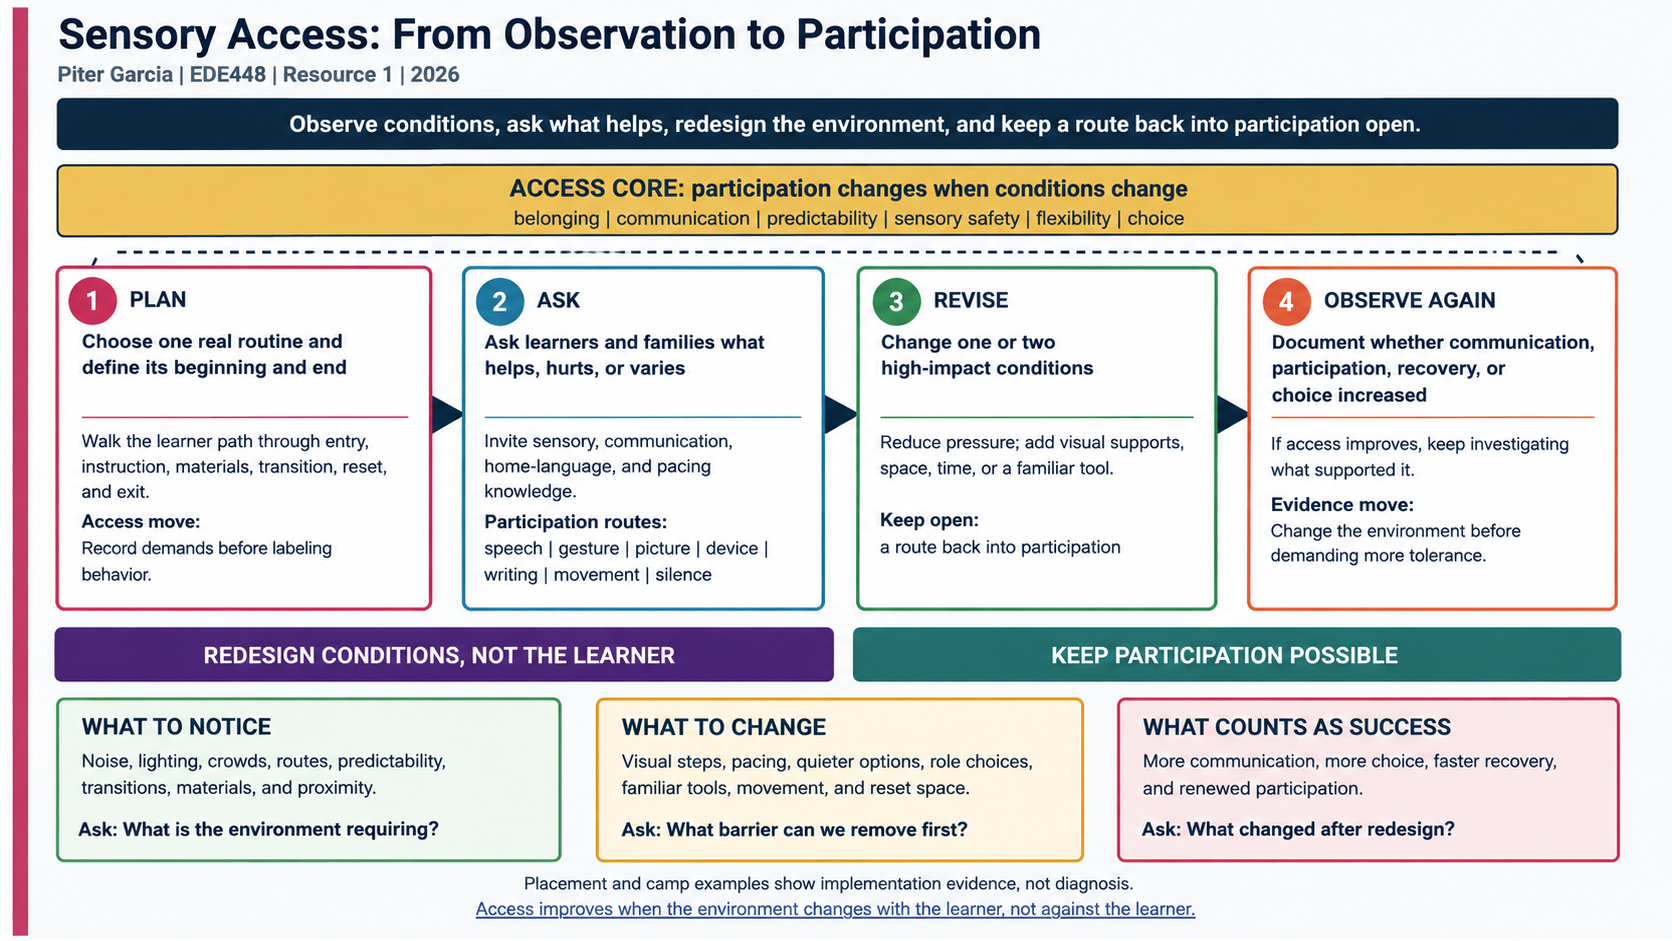
\includegraphics[
  width=1.0\textwidth,
  keepaspectratio
]{assets/artifact-previews/observation_to_participation.png}

\parbox{1.0\textwidth}{\centering\scriptsize
\textbf{\color{DeepNavy}Sensory Access: From Observation to Participation.}
The framework connects observation, learner and family input, environmental redesign, and renewed observation so that changes in communication and participation guide the next instructional decision.}
\end{center}

\adaptationbox{Sensory support is individual and can change across activity, time, fatigue, pain, and experience. The goal is not to make learners tolerate more, but to adjust conditions while protecting communication, participation, and belonging.}

\sourcebox{\scriptsize Guggenheim sensory-environment course resource \citep{guggenheimSensory}; Michigan Developmental Disabilities Institute checklist \citep{michigan2025sensory}.}
\resourceheading{2}{Many Ways to Be a Good Classmate}{Autism inclusion, peer culture \& social-emotional learning}{Teachers, specialists \& families}{Module 1 taught Kit for Kids lesson and a documented Grade 2 technology routine}

\vspace{-0.5cm}
\toolsection{What This Resource Is}

Environmental access is only part of inclusion; peer culture can either preserve or undo it. This ten-minute peer-education lesson turns ``be kind'' into four observable actions: \textsc{invite, wait, ask, and respect}. It draws on the Organization for Autism Research (OAR) Kit for Kids, the \textit{What's Up with Nick?} booklet, and grade-banded friendship tips \citep{oar2026kit,oar2026nick,oar2026tips}. The lesson normalizes different ways of communicating, learning, moving, regulating, and participating. Students need language for helping without taking over, waiting without rushing, offering space without excluding, and accepting communication through speech, writing, pictures, AAC, gesture, movement, or silence. During camp, peer support sometimes looked similarly ordinary: continuing shared work, giving another person room, and keeping a route back into participation open rather than making that person's behavior the focus \citep{campEvidence2026}.

\toolsection{Ten-Minute Lesson Sequence}

\small
\renewcommand{\arraystretch}{1.15}
\setlength{\tabcolsep}{5pt}

\begin{tabularx}{\textwidth}{
>{\bfseries\RaggedRight\arraybackslash}p{0.75in}
>{\RaggedRight\arraybackslash}p{1.60in}
>{\RaggedRight\arraybackslash}X}

\rowcolor{PrimaryRed}
\color{white}Time &
\color{white}Move &
\color{white}Teacher Language and Student Action \\

0--2 min & Preview &
Show \textit{first/next/last}. ``Brains and bodies work in different ways. Good classmates help everyone participate without asking anyone to explain private information.'' \\

\rowcolor{SoftGray}
2--4 min & Teach &
Introduce the four actions below with one example and one nonexample each. \\

4--8 min & Practice &
Present one authentic classroom scenario. Pairs name a barrier, choose an action, and explain how it preserves choice. \\

\rowcolor{SoftGray}
8--10 min & Commit/close &
Students complete: ``One way I can support a classmate is...'' by speaking, writing, drawing, pointing, or passing and returning later. \\

\end{tabularx}

\normalsize

\toolsection{Four Peer Actions}

\setlength{\tabcolsep}{5pt}

\begin{tabularx}{\textwidth}{
>{\bfseries\color{DeepNavy}\RaggedRight\arraybackslash}p{0.72in}
>{\RaggedRight\arraybackslash}X
>{\RaggedRight\arraybackslash}X}

Invite &
Offer a role, seat, material, or turn without forcing a response. &
``Would you like to test, point, watch first, or choose another role?'' \\

\rowcolor{SoftGray}
Wait &
Leave processing time and keep the floor available. &
Count silently; do not repeat the question faster or answer for the person. \\

Ask &
Ask what support helps rather than guessing from a diagnosis or behavior. &
``Do you want help, more time, space, or a different way?'' Include ``something else.'' \\

\rowcolor{SoftGray}
Respect &
Protect communication tools, sensory needs, boundaries, breaks, privacy, and refusal. &
Do not grab a device, require eye contact, disclose a diagnosis, or make support conditional on compliance. \\

\end{tabularx}

\vfill

\begin{center}
\begin{tikzpicture}[
action/.style={draw=DeepNavy, rounded corners=2pt, minimum width=1.45in,
minimum height=0.60in, align=center, font=\scriptsize, inner sep=4pt},
next/.style={-{Latex[length=1.7mm]}, line width=0.7pt, draw=PrimaryRed}
]
\node[action, fill=SoftBlue] (invite) {\textbf{INVITE}\\offer a real route};
\node[action, fill=SoftGold, right=0.13in of invite] (wait) {\textbf{WAIT}\\keep the floor open};
\node[action, fill=SoftGreen, right=0.13in of wait] (ask) {\textbf{ASK}\\support, do not guess};
\node[action, fill=SoftRose, right=0.13in of ask] (respect) {\textbf{RESPECT}\\tools, boundaries, refusal};

\draw[next] (invite) -- (wait);
\draw[next] (wait) -- (ask);
\draw[next] (ask) -- (respect);

\node[font=\scriptsize\bfseries, text=DeepNavy,
below=0.09in of $(wait.south)!0.5!(ask.south)$]
{Choice stays with the learner};
\end{tikzpicture}
\end{center}

\newpage
\toolsection{Practice Scenario}

During a technology activity, one student has entered the program while several peers are still stuck. Another student is new to the routine. Ask: \textit{What barrier is present? What can a peer do without taking over? How can the person decline help?} Strong responses include showing one click, giving time to try, lowering voice volume, keeping the Chromebook in the learner's control, including the new student as part of the class, and accepting ``no thanks.''

\begin{center}
\colorbox{SoftGreen}{\parbox{0.93\textwidth}{\small
\textbf{Documented student evidence from the taught lesson:} One Grade 2 student proposed showing the next click without grabbing a classmate's Chromebook. Another said a new person should not be made to feel left out. These responses show students applying \textit{wait}, \textit{respect}, and \textit{invite} inside the actual technology routine.
}}
\end{center}

Use the same lesson before robotics, group building, recess transitions, digital publishing, or showcases. Revisit one action during the real routine; inclusion is learned through repeated practice, not one awareness event.

\reflectionbox{I taught this ten-minute lesson immediately before a partner-based Grade 2 coding and robotics routine. The strongest design move was locating support inside the activity rather than giving an abstract lecture: students had to decide how to help classmates enter a program without taking over and how to include a visitor in the classroom community \citep{placement2026robotics}. Ten minutes established shared language, but repeated practice is necessary before the four actions become a dependable peer norm. In Puzzle Plan terms, peer behavior becomes part of the access context; EQUITAS asks whether helping preserves the other student's authorship and right to decline.}

\adaptationbox{Ten minutes introduces shared language but cannot represent the full range of autistic experience. Pair OAR's educator material with autistic-authored perspectives when developmentally appropriate, adapt examples to age and culture, and monitor whether peers begin to police difference under the banner of helping. Adult redesign remains necessary; peer kindness cannot compensate for inaccessible schedules, noise, tools, or instruction.}

\begin{center}

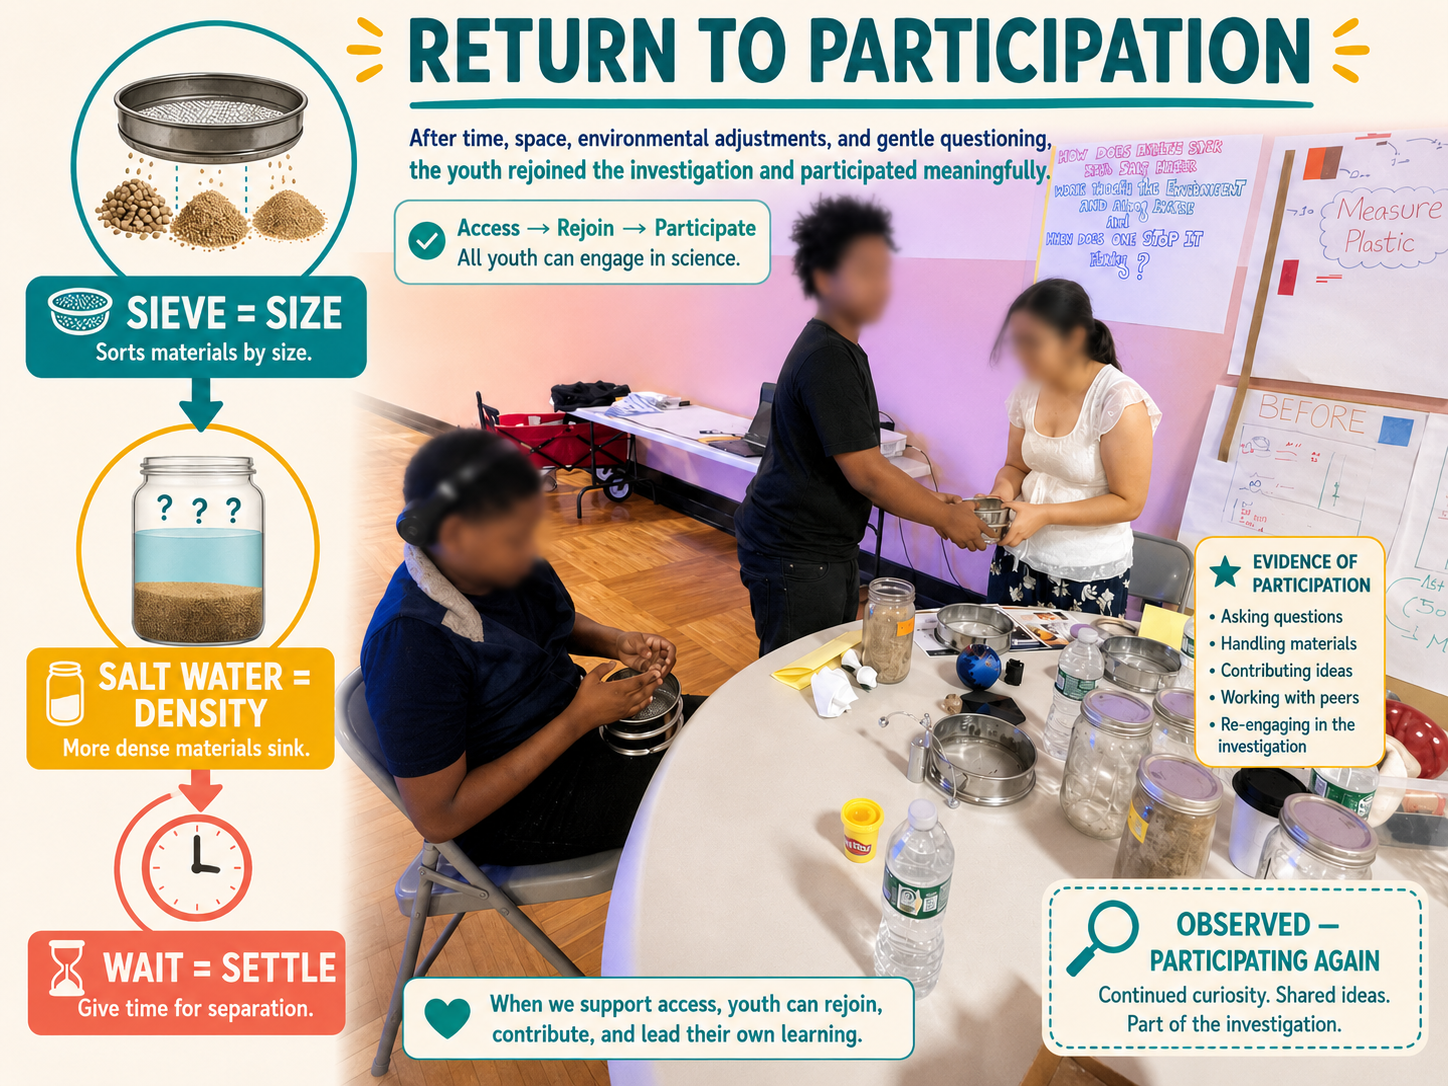
\includegraphics[
  width=0.75\textwidth,
  keepaspectratio
]{assets/artifact-previews/Return to Participation.png}

\parbox{0.90\textwidth}{\centering\scriptsize
\textbf{\color{DeepNavy}Peer Support in Practice.}
Camp practice illustrates the same peer norm: support can mean continuing shared work, giving a classmate room, and keeping a genuine route back into the investigation. The aim is not to manage another learner's behavior, but to preserve belonging without taking over.}

\end{center}

\sourcebox{\scriptsize OAR Kit for Kids \citep{oar2026kit}, \textit{What's Up with Nick?} \citep{oar2026nick}, and Friendship Tip Sheets \citep{oar2026tips}.}
\resourceheading{3}{PTR Evidence-to-Support Planning Guide}{Positive \& proactive behavior support}{Teachers, families \& support teams}{Module 2 Prevent--Teach--Reinforce assignment and a non-identifying placement event}

\vspace{-0.5cm}
\toolsection{What This Resource Is}

Prevent--Teach--Reinforce (PTR) is a team-based process for defining a concern observably, examining context and possible function, designing a linked plan, and reviewing both outcomes and implementation fidelity \citep{dunlap2019ptr}. This guide keeps observation, inference, hypothesis, and support decisions separate. Teams gather multiple observations, build a provisional hypothesis, and then link supports to what the evidence suggests. PTR supports communication and behavior when \textit{Prevent}, \textit{Teach}, and \textit{Reinforce} address the same access problem. Prevention changes conditions that make communication difficult. Teaching creates a safer or more efficient way to express the same need. Reinforcement makes that communication effective through a meaningful outcome rather than rewarding surface compliance.

\toolsection{Use This Guide Before Writing a Plan}
% \small
\renewcommand{\arraystretch}{1.0}
\setlength{\tabcolsep}{2.5pt}

\begin{longtable}{
>{\bfseries\RaggedRight\arraybackslash}p{0.70in}
>{\RaggedRight\arraybackslash}p{1.70in}
>{\RaggedRight\arraybackslash}p{2.00in}
>{\RaggedRight\arraybackslash}p{2.52in}}

\tableheaderfour{Step}{Record}{Ask}{Example Support}

Observe &
Actions, words, timing, task, tools, people, sensory conditions, and adult responses &
What can another observer verify? What remains unknown? &
``Adult reached for laptop; learner raised voice and held device.'' \\

\rowcolor{SoftGray}
Hypothesize &
A provisional relationship among conditions, communication, and outcome &
What other explanations fit? What student/family knowledge is missing? &
Familiar tool may support predictability, regulation, continued access, or something else. \\

Prevent &
Barrier changes before escalation &
Can the transition be previewed, modeled, overlapped, or chosen? &
Visible warning; laptop beside blocks; observe-first or partner-start option. \\

\rowcolor{SoftGray}
Teach &
A message or participation route that serves the same purpose &
Can the learner say it through speech, writing, gesture, AAC, or pointing? &
\textit{Not yet, more time, keep this with me, show me, help, break.} \\

Reinforce &
Natural response that makes the new route reliable &
Does the message change what happens when safety allows? &
More time occurs; familiar tool remains; learner enters through a chosen route. \\

\rowcolor{SoftGray}
Review &
Student outcomes and adult implementation &
Was the option available, recognized, honored, and useful? &
Track communication, participation, distress, trust, access, and fidelity. \\
\end{longtable}

\normalsize
\begin{center}

\begin{minipage}[c]{0.70\textwidth}
\centering
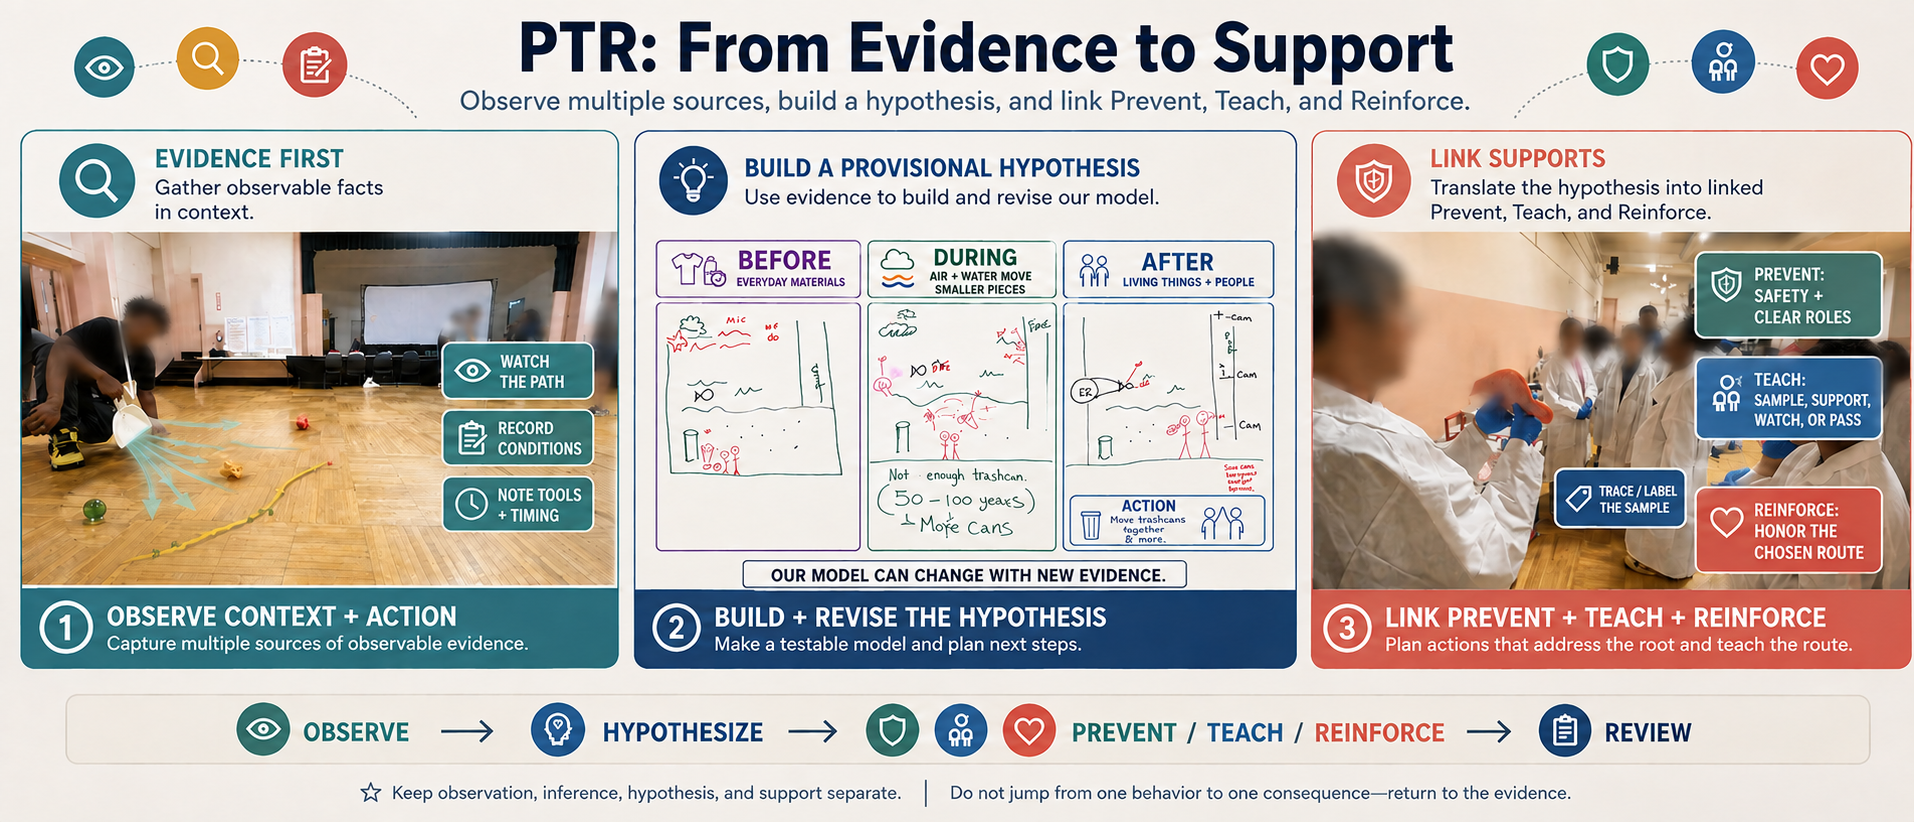
\includegraphics[
  width=0.90\linewidth,
  keepaspectratio
]{assets/artifact-previews/from_evidence_to_support.png}
\end{minipage}
\hfill
\begin{minipage}[c]{0.29\textwidth}
% \scriptsize
\RaggedRight
{\centering\bfseries\color{DeepNavy} From Evidence to Support.\par}
{\centering Camp practice illustrates the same planning logic: observable conditions and actions provide evidence, multiple pieces inform a provisional model, and that model guides linked supports. New evidence then returns the team to review and revision.\par}
\end{minipage}

\end{center}

\newpage
\toolsection{Completed Assignment Artifact: Appendix 4.1 Snapshot}

A public companion to the official checklist made uncertainty visible instead of filling gaps with assumptions:

\small
\renewcommand{\arraystretch}{1.13}
\setlength{\tabcolsep}{5pt}

\begin{tabularx}{\textwidth}{
>{\bfseries\RaggedRight\arraybackslash}p{1.36in}
>{\RaggedRight\arraybackslash}X}

\rowcolor{PrimaryRed}
\color{white}Checklist Area &
\color{white}Evidence-Supported Entry \\

Most associated routine &
Transition from familiar laptop use to a hands-on blocks activity; attempted device removal immediately preceded protest. \\

\rowcolor{SoftGray}
Least associated routine &
Unknown. Increased participation after the laptop remained is a response-to-support observation, not a stable pattern. \\

Provisional hypothesis &
Abrupt removal may have made the transition harder; preserving laptop access may have supported predictability, regulation, continuity, communication, preferred activity, or another function. \\

\rowcolor{SoftGray}
Evidence still needed &
Learner and family perspective; repeated observations; current IEP supports; latency, communication route, adult fidelity, and participation across conditions. \\

\end{tabularx}

\normalsize

Implementation commitments are to build the team with the learner and family, collect repeated baseline evidence, link all three PTR components to one hypothesis, include adult and environmental actions, and decide what evidence will trigger a keep/change/stop decision.

\begin{center}
\begin{minipage}[c]{0.62\textwidth}
\centering
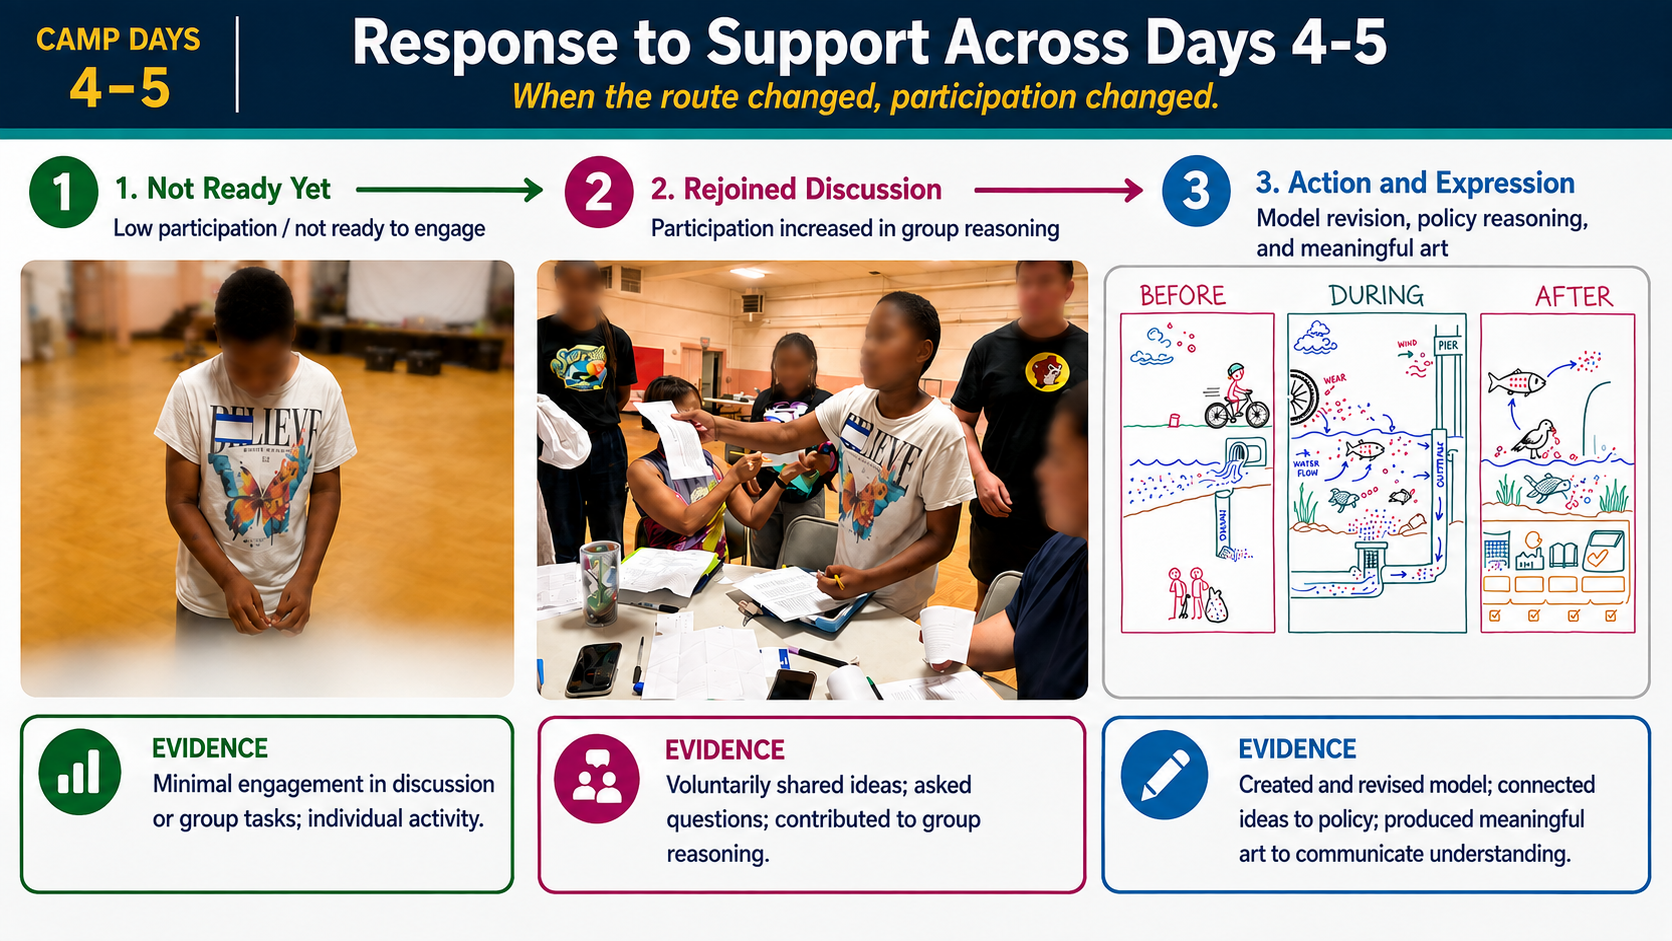
\includegraphics[
  width=\linewidth,
  keepaspectratio
]{assets/artifact-previews/response_to_support_across_days_4_5.png}
\end{minipage}
\hfill
\begin{minipage}[c]{0.37\textwidth}
% \scriptsize

{\centering\bfseries\color{DeepNavy} Evidence Boundary.\par}

{\centering The camp sequence documents increased participation after support changed: from not being ready to engage, to group reasoning, and then to action and expression. It shows a response to support over time, not a confirmed behavioral function.\par}

\end{minipage}
\end{center}

Constructing communicative competence requires more than presuming it: educators must make useful communication available and consequential throughout the day \citep{jorgensen2018competence}. A learner should not have to surrender a familiar support, become quiet, make eye contact, or follow an adult's preferred schedule to demonstrate success. Gardner's first-hand report warns that apparently effective intervention can still produce masking, shame, or weaker boundaries when conformity is the real outcome \citep{gardner2017firsthand}.

\reflectionbox{The Module 2 case began with one documented transition: an adult attempted to remove a familiar laptop before a blocks activity; after the either--or condition was removed, the learner joined the building activity while keeping the laptop nearby. This does not establish a behavioral function or a universal laptop intervention. Like the camp sequence above, it shows why changes in conditions and participation belong in the evidence record. Puzzle Plan keeps those conditions visible; EQUITAS keeps the learner and family able to contest the team's interpretation. ``Unknown'' is an accountable finding when the data do not support a conclusion.}

\adaptationbox{PTR can be misused when teams select compliance goals, ignore communication modes, or count only student behavior. Review cultural and family meaning, sensory and health conditions, language access, and whether the learner can disagree with the team's interpretation. If visible behavior decreases while communication, trust, participation, or quality of life also decreases, the plan is not positive and should be revised.}

\sourcebox{PTR second edition \citep{dunlap2019ptr}; communication competence \citep{jorgensen2018competence}; first-hand intervention perspectives \citep{gardner2017firsthand}.}
\resourceheading{4}{30-Second Student Video Memo}{Student voice, formative communication, SEL \& behavior-as-communication\par}{Students, teachers, families \& support teams}{Implemented EDU486 post-activity video memos and de-identified source transcripts}

\vspace{-0.5cm}
\toolsection{The Existing Camp Artifact}

PTR improves how adults interpret evidence; the 30-second memo changes who gets to author that evidence. During the Invisible Invaders camp, youth were invited after an activity to explain in their own words what they did, how they experienced it, what they learned or confirmed, and what they wanted to investigate next. The reviewed Field Friday source index preserves a 43-second post-activity memo in which a youth described the sand-sampling work as hands-on, said they liked it, distinguished new learning from something confirmed, and connected the activity to a larger exposure question \citep{campEvidence2026}. This is a communication support because the learner, not an adult behavior rating, authors the first account of the activity. It also supports social-emotional learning by giving students a routine for recognizing how an experience affected them, naming what helped or did not help, and communicating what they want next. Preferences, confusion, sensory responses, questions, and change requests can become visible before adults reduce them to engagement, compliance, or disruption. The memo gives the next teacher, family member, or collaborator evidence for redesign.

\toolsection{Four Prompts, One Student-Owned Record}

Use the memo after each major activity while keeping the time, mode, and decision to participate flexible.

\small
\renewcommand{\arraystretch}{1.00}
\setlength{\tabcolsep}{3pt}

\begin{tabularx}{\textwidth}{
>{\bfseries\RaggedRight\arraybackslash}p{0.90in}
>{\RaggedRight\arraybackslash}p{2.35in}
>{\RaggedRight\arraybackslash}X}

\rowcolor{PrimaryRed}
\color{white}Memo Move &
\color{white}Open Prompt &
\color{white}What It Makes Visible \\

Do &
What did you do, make, notice, or contribute? &
Activity, role, participation route, and evidence the learner considers important \\

\rowcolor{SoftGray}
Feel / experience &
How did it feel? What did you like, dislike, or want changed? &
Emotional awareness, joy, discomfort, sensory access, pacing, relationships, and task fit without guessing from behavior \\

Learn / confirm &
What did you learn? Did anything confirm, challenge, or change an idea? &
Content understanding, prior knowledge, model revision, uncertainty, and metacognition \\

\rowcolor{SoftGray}
Continue &
What question do you have, or what should we investigate next? &
Curiosity, self-advocacy, agency, unfinished thinking, and the next storyline or support decision \\

\end{tabularx}

\normalsize

The facilitator asks once, waits, and follows the learner's language rather than supplying the answer. ``Nothing yet,'' ``I did not like that,'' ``pass,'' and ``delete it'' are valid responses. A memo may be video, audio, AAC, text, drawing plus dictated caption, photographs selected by the learner, or a partner-supported interview. Emotional learning here is not about producing a preferred feeling; it is about recognizing an experience, communicating it, and having that communication matter.

\begin{center}

{\scriptsize\bfseries\color{DeepNavy}From Student Memo to the Next Opportunity}\par


\begin{tikzpicture}[
memo/.style={draw=DeepNavy, rounded corners=2pt, minimum width=1.0in,
minimum height=0.10in, align=center, font=\tiny, inner sep=1pt},
next/.style={-{Latex[length=1.5mm]}, line width=0.15pt, draw=PrimaryRed}
]
\node[memo, fill=SoftBlue] (activity) {\textbf{ACTIVITY}\\work remains present};
\node[memo, fill=SoftGold, right=0.12in of activity] (voice) {\textbf{STUDENT MEMO}\\do / feel / learn / continue};
\node[memo, fill=SoftGreen, right=0.12in of voice] (review) {\textbf{REVIEW MEANING}\\keep, edit, correct, delete};
\node[memo, fill=SoftRose, right=0.12in of review] (action) {\textbf{CHANGE NEXT MOVE}\\pace, material, question, route};

\draw[next] (activity) -- (voice);
\draw[next] (voice) -- (review);
\draw[next] (review) -- (action);
\end{tikzpicture}

\parbox{1.0\textwidth}{\centering\tiny
\textit{Implemented evidence loop.}
The reviewed archive preserves a 43-second post-activity memo; its value is not the recording itself but whether the student's reflection---including emotional experience---can alter the next opportunity.}

\end{center}

\reflectionbox{\textbf{Artifact proof and SEL connection:} the reviewed Field Friday source index preserves 18 original recordings and de-identified transcript records, including a 43-second post-activity memo. Adjacent records preserve another youth's investigation question and a sampling-site hypothesis. More importantly, the memo preserved the learner's own account of what they did, how they experienced it, what they understood, and what they wanted to pursue next. That makes emotional learning consequential: recognizing and communicating a feeling or preference can become evidence for changing the next activity. Planning is not used as proof of implementation; reviewed recordings and transcripts document the routine, while later reflection documents interpretation.}

\newpage
\toolsection{Ready-to-Reuse Memo Workflow}

\begin{enumerate}
  \item \textbf{Ask permission before recording.} Name the audience and offer a non-camera route.
  \item \textbf{Keep the activity present.} Let the learner hold, point to, photograph, or revisit the work.
  \item \textbf{Use the four prompts as options.} Do not require a polished answer to every question.
  \item \textbf{Let the student review.} Keep, redo, edit, caption, restrict, or delete the memo.
  \item \textbf{Preserve identity.} Transcribe accurately; retain home language, AAC wording, pauses, and uncertainty.
  \item \textbf{Tag for action, not judgment.} Record the activity, access route, preference or barrier, learning or confirmation, question, and requested change.
  \item \textbf{Close the loop.} Show what changed in the next activity and invite learners to correct the interpretation.
\end{enumerate}

\toolsection{Communication-to-Support Record}

\small
\renewcommand{\arraystretch}{1.08}
\setlength{\tabcolsep}{4pt}

\begin{tabularx}{\textwidth}{
>{\bfseries\RaggedRight\arraybackslash}p{1.35in}
>{\RaggedRight\arraybackslash}X}

\rowcolor{MidTeal}
\color{white}Record Field &
\color{white}Reviewed Camp Example \\

Activity and contribution &
Prepared sand samples for investigation; described the work as hands-on \\

\rowcolor{SoftGray}
Student experience &
Communicated liking the activity; no emotion is inferred beyond the student's own response \\

Learning / confirmation &
Distinguished confirmation of prior knowledge from wholly new learning \\

\rowcolor{SoftGray}
Question / next move &
Connected the activity to a broader exposure question; an adjacent memo generated a question for a community worker \\

Adult action &
Preserve hands-on investigation, answer or carry forward the question, and avoid turning the memo into a recall test \\

\rowcolor{SoftGray}
Evidence boundary &
Automatic transcript supports a de-identified summary; quotation and speaker identity require source-audio review \\

\end{tabularx}

\normalsize

\toolsection{Puzzle Plan and EQUITAS in Practice}

The Puzzle Plan refuses to let an adult observation, behavior count, photograph, or diagnosis stand alone. The memo adds lived experience and student interpretation to the evidence system. EQUITAS then asks whose account shapes tomorrow's lesson, what the camera could not capture, whether prompting narrowed the answer, and whether the learner can control the record. A memo matters only when youth words can change pacing, materials, access routes, questions, or what adults communicate about them.

\begin{center}
\begin{minipage}[c]{0.50\textwidth}
\centering
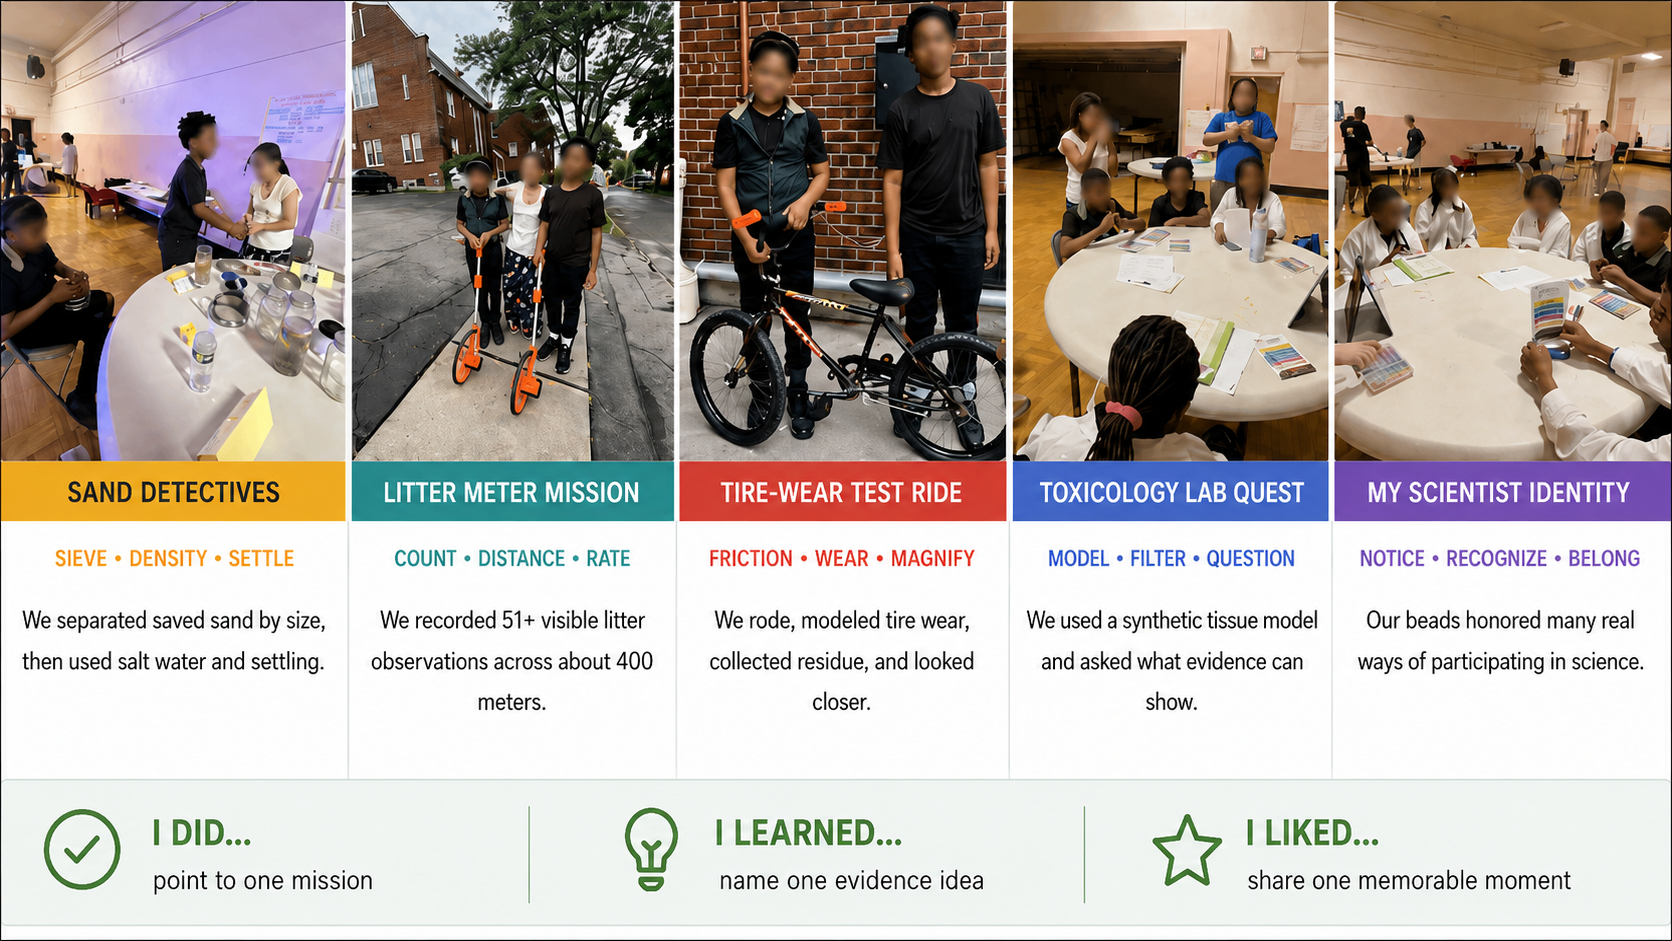
\includegraphics[
  width=0.96\textwidth,
  keepaspectratio
]{assets/artifact-previews/five_mission_learning_showcase.png}
\centering\scriptsize
{
\bfseries\color{DeepNavy}
Keep the Activity Present.\par
}
The camp recap kept the week's actual activities visible while youth reflected through \textit{I did}, \textit{I learned}, and \textit{I liked}. A learner could point, speak, or use the visual instead of recording a video. The memo is therefore one communication route, not the required route.\par
\end{minipage}
\hfill
\begin{minipage}[c]{0.49\textwidth}
{
\adaptationbox{A camera can create performance pressure or surveillance. Never infer private emotion from appearance, fluency, silence, or refusal. Do not post, send, or retain a memo beyond the agreed audience and purpose. Provide captioning, translation, AAC access, processing time, and a private or asynchronous option. Day 5 had photographs and a same-session transcript but no source video; this evidence system names that gap.}
}
\sourcebox{\scriptsize Video-memo archive \citep{campEvidence2026}; rich communicative environments \citep{downing2015classroom}; communication and behavior \citep{peckhamhardin2015behavior}; communicative competence \citep{jorgensen2018competence}.}
\end{minipage}
\end{center}

\endinput
\resourceheading{5}{Every-Day Personalized Science Souvenir}{Student learning portrait, recognition, memory \& communication continuity\par}{Students, families, teachers \& camp partners}{Implemented EDU486 personalized souvenirs, student memos, and reviewed activity evidence}

\vspace{-0.5cm}
\toolsection{The Existing Camp Artifact}

The video memo preserves an immediate learner account, and the personalized souvenir carries that account into memory and family conversation. The Invisible Invaders team paired a child-forward activity image with the learner's contribution, field-memo thinking, science moves, traceable evidence, why the learning mattered, and what remained unconfirmed. The visual message was direct: \textit{``This is you doing science.''} The product recognized authorship without turning a photograph into proof of understanding \citep{campEvidence2026}. A learner could revisit the day's experiences, point to a mission, retell what they did or learned, and use the visual record when words alone were difficult. The reviewed archive preserves completed souvenirs for every day, including one Day 5 image for each assigned youth.

\toolsection{The Completed Souvenir}

\begin{center}

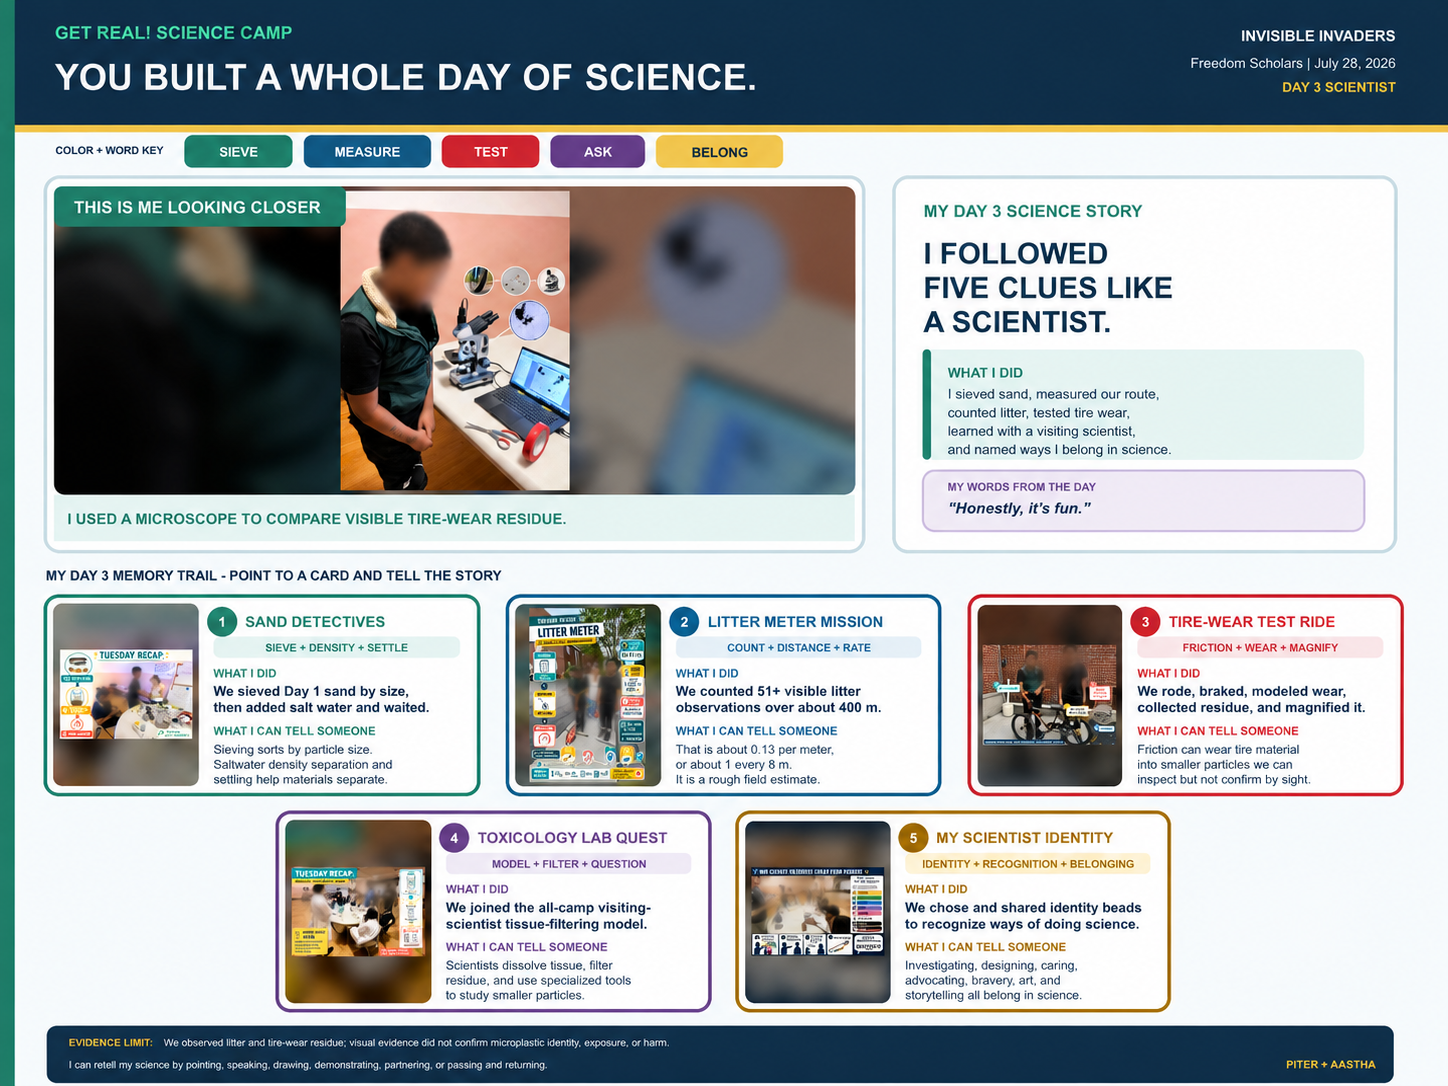
\includegraphics[
  width=0.92\textwidth,
  keepaspectratio
]{assets/artifact-previews/souvenir-day3-example.png}

\parbox{0.92\textwidth}{\centering\small
\textbf{\color{DeepNavy}Public-safe Day 3 souvenir.}
The completed artifact brings together the learner in action, a transcript-grounded science story, five activity memories, the learner's own words, multiple communication routes, and an explicit evidence limit. It functions as both recognition and a reusable memory aid for retelling the learning to teachers, families, or partners.}

\end{center}

\newpage
\toolsection{Build One After Each Activity Day}

\begin{enumerate}
	\item \textbf{Assemble the evidence set:} activity record, student memo or artifact, reviewed photographs, team notes, and the learning goal.
	\item \textbf{Start with the learner's contribution:} identify what the young person chose, noticed, made, changed, asked, explained, or helped the group do.
	\item \textbf{Separate evidence levels:} mark exact words, artifact language, documented action, team-level evidence, adult interpretation, and uncertainty.
	\item \textbf{Select and compose together:} choose the image and idea; add the science story, moves, evidence, significance, and limit; offer caption, translation, retake, and no-photo routes.
	\item \textbf{Review, share, and reuse:} check identity, attribution, quotation, permission, and audience; next day, invite the learner to point, tell, correct, extend, or decline the story.
\end{enumerate}

\toolsection{Evidence-to-Action Review}

% \small
\renewcommand{\arraystretch}{1.00}
\setlength{\tabcolsep}{4pt}
\begin{tabularx}{\textwidth}{>{\bfseries\RaggedRight\arraybackslash}p{1.20in} >{\RaggedRight\arraybackslash}p{2.65in} >{\RaggedRight\arraybackslash}X}
\rowcolor{MidTeal}
\color{white}Souvenir Signal & \color{white}Interpret Carefully & \color{white}Adult Follow-Through \\
Student words & Preserve the learner's meaning; do not polish uncertainty away & Reuse the question, preference, or connection in the next lesson \\
\rowcolor{SoftGray}
Documented action & Participation may be visible without proving the learner's full understanding & Ask the learner what the action meant and offer another way to demonstrate thinking \\
Preference or boundary & Liking, refusing, passing, or requesting change is communication & Change material, role, pace, sensory route, or audience when feasible \\
\rowcolor{SoftGray}
Team contribution & Credit individual influence without claiming the whole team's product & Name both the student's move and the shared work \\
Evidence gap & ``Still to test'' is part of scientific competence, not failure & Carry the uncertainty into the recap and next investigation \\
\end{tabularx}
\normalsize

\toolsection{Puzzle Plan and EQUITAS in Practice}

The Puzzle Plan joins the student's account, observable action, work product, team record, and scientific context without allowing one piece to define the learner. EQUITAS asks who selected the image and story, whose language was edited, whose quieter contribution disappeared, and whether the artifact changes adult memory while celebrating the child. Used this way, the souvenir supports communication and behavior by making competence, boundaries, curiosity, and participation routes visible before a deficit story replaces them.

\reflectionbox{\textbf{Artifact proof:} the private handoff contains reviewed personalized souvenir PDFs, activity images, and source-video indexes. Day 5 is explicitly limited to photographs and a same-session clean transcript; it has no source video. The souvenir system preserves that distinction and never upgrades an attractive visual into stronger evidence \citep{campEvidence2026}.}

\adaptationbox{A souvenir can become a reward, comparison chart, or privacy violation if adults control every choice. Never reserve it for compliance or fluent speech. Offer photo-free, name-free, home-language, AAC, audio, tactile, or student-created versions. Use identifiable copies only within the program's signed consent and approved educational audience.}

\sourcebox{Personalized souvenir archive \citep{campEvidence2026}; communicative competence \citep{jorgensen2018competence}; first-hand perspectives \citep{gardner2017firsthand}.}
\resourceheading{6}{AAC Tool Selection and Implementation Guide}{Augmentative \& alternative communication\par}{Teachers, families, speech-language pathologists \& support teams}{Module 3 AAC Review, Grade 2 IGNITE curriculum, and TD Snap as a worked example}

\vspace{-0.5cm}
\toolsection{What This Resource Is}

This is a decision guide for evaluating an AAC tool as one part of a multimodal communication system. AAC includes aided and unaided methods, and eligibility should not depend on age, cognitive score, or mastery of prerequisite milestones \citep{ashaAAC,mirenda2015aids}. The core question is not whether a student can use a device in isolation, but whether the communicator can access meaningful vocabulary, participate across real routines, rely on responsive partners, and influence what happens next. TD Snap is the worked example because its current product information describes multiple page sets and access routes, including symbol-supported and text-based options, touch, switch scanning, and eye-gaze-compatible use \citep{tobii2026tdsnap}. Those features create possibilities; they do not replace individualized feature matching, trial use, training, technical support, funding review, or communicator consent. 
\begin{figure}[H]
\centering
\begin{tikzpicture}[
	node distance=0.06in,
	stage/.style={
		draw=DeepNavy,
		rounded corners=2pt,
		minimum width=1.22in,
		minimum height=0.34in,
		text width=1.12in,
		align=center,
		font=\tiny,
		inner sep=2pt
	},
	flow/.style={
		-{Latex[length=1.1mm]},
		line width=0.6pt,
		draw=PrimaryRed
	}
]

\node[font=\scriptsize\bfseries, text=DeepNavy] (title)
	{TD Snap in a Multimodal Communication System};

\node[stage, fill=SoftGold, below=0.07in of title] (intent)
	{\textbf{STUDENT MEANING}\\comment, question, refuse, repair};

\node[stage, fill=SoftBlue, right=of intent] (access)
	{\textbf{ACCESS ROUTE}\\touch, gaze, switch, gesture};

\node[stage, fill=SoftRose, right=of access] (tool)
	{\textbf{TOOL / DISPLAY}\\TD Snap, board, visual model};

\node[stage, fill=SoftGray, right=of tool] (partner)
	{\textbf{PARTNER}\\model, wait, notice, confirm};

\node[stage, fill=SoftGold, right=of partner] (agency)
	{\textbf{AGENCY}\\message changes what happens};

\draw[flow] (intent) -- (access);
\draw[flow] (access) -- (tool);
\draw[flow] (tool) -- (partner);
\draw[flow] (partner) -- (agency);

\node[
	draw=MidTeal,
	fill=SoftGreen,
	rounded corners=2pt,
	below=0.10in of tool,
	text width=6.25in,
	align=center,
	font=\tiny,
	inner sep=3pt
] (conditions)
{\textbf{Conditions that travel with the system:}
preference + consent $\bullet$ identity + language $\bullet$ low-tech backup $\bullet$ partner + technical support};

\node[
	draw=PrimaryRed,
	dashed,
	rounded corners=2pt,
	below=0.06in of conditions,
	text width=6.25in,
	align=center,
	font=\tiny,
	inner sep=3pt
] (equitas)
{\textbf{EQUITAS test:}
Can the student choose, refuse, comment, question, repair, revise, participate, and influence what happens next?
If not, revise the system---not the student.};

\end{tikzpicture}

\vspace{-0.05in}
\caption{\scriptsize
Communication becomes access-to-agency when meaning, access, tools, partners, and meaningful outcomes stay connected.}
\label{fig:td-snap-system}
\end{figure}

\vspace{-0.2in}
The same principle appeared in the Grade 2 IGNITE curriculum through shared visual models. In camp, students built a \textit{Before / During / After} pathway model to explain how tiny plastic pieces move through the environment and into living bodies. That artifact matters here because it shows that communication is not limited to speech or a single app: a student may comment, question, revise, point, explain, or co-construct meaning through a shared visual, partner prompting, gesture, writing, symbols, or a high-tech AAC system. AAC tool selection should therefore be judged by whether it expands participation and meaning-making, not by whether it makes a student look more conventionally verbal.

\toolsection{Shared Visual Model as a Communication Support}

\begin{center}
\begin{minipage}[c]{0.68\textwidth}
\centering
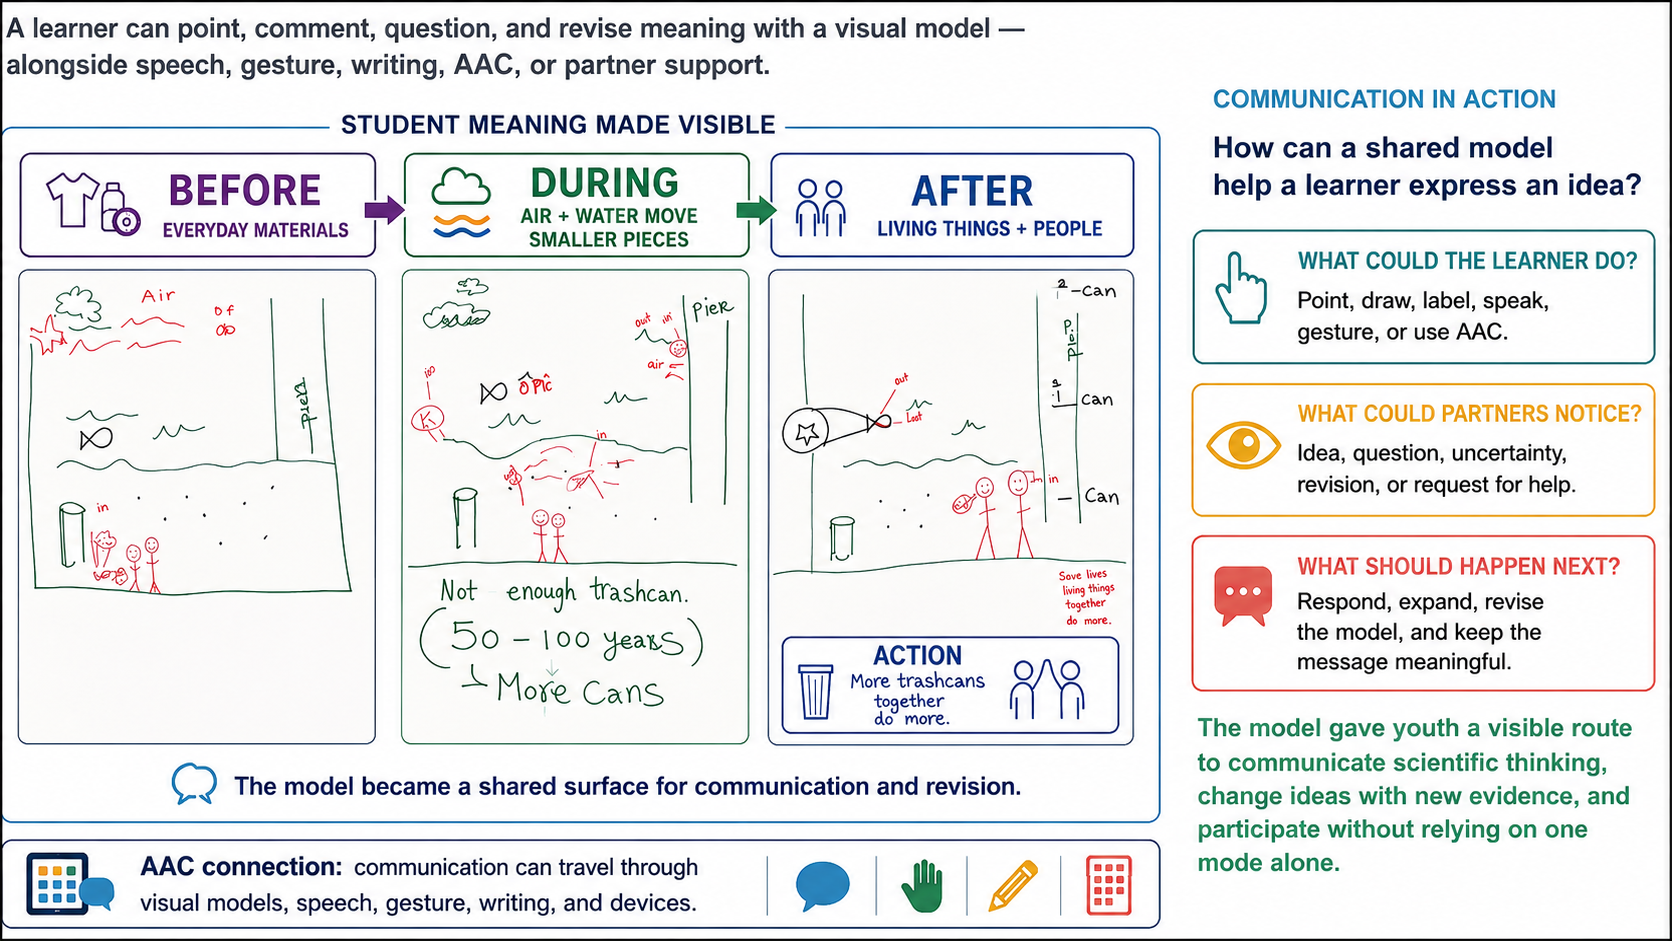
\includegraphics[
  width=1.0\linewidth,
  keepaspectratio
]{assets/artifact-previews/shared_visual_model_for_communication.png}
\end{minipage}
\hfill
\begin{minipage}[c]{0.29\textwidth}
\scriptsize

{\centering\bfseries\color{DeepNavy} Shared model, shared meaning.\par}
{\centering
The camp model functioned as a communication support because students could point to, revise, and explain ideas through a visible pathway rather than relying on speech alone. The three student-authored panels remained intact, while added prompts highlighted communicative purposes: naming the question, identifying what they thought, deciding what evidence was needed, and stating what should change.\par
}

{\centering
This makes the visual relevant to AAC: it supported commenting, questioning, revising, and action-planning through multiple response routes.\par
}
\end{minipage}
\end{center}




\newpage
\toolsection{AAC Selection and Trial Matrix}

\small
\renewcommand{\arraystretch}{1.0}
\setlength{\tabcolsep}{4pt}

\begin{longtable}{
>{\bfseries\RaggedRight\arraybackslash}p{1.0in}
>{\RaggedRight\arraybackslash}p{3.00in}
>{\RaggedRight\arraybackslash}p{2.87in}}

\tableheaderthree{Domain}{Questions for the Team}{Evidence During Trial}

Communicator &
What modes, languages, identities, interests, relationships, and messages matter now? What does the person accept, choose, or reject? &
Initiations, message range, preference, fatigue, refusal, repair, and whether the learner chooses among available communication routes \\

\rowcolor{SoftGray}
Access &
What routes are usable: touch, pointing, eye gaze, switch, scanning, gesture, positioning, vision, hearing, sensory, or motor access? &
Accuracy and effort across locations, materials, body positions, time of day, and changing access needs \\

Vocabulary \& representation &
Are core, activity, identity, bilingual, academic, social, humor, refusal, pain, and repair language available? Can meaning also be supported through symbols, photos, text, or shared visual models? &
The learner comments, questions, refuses, repairs, and revises ideas rather than using the system only to make requests \\

\rowcolor{SoftGray}
Partners &
Who models, waits, notices, confirms, repairs, and responds? Can partners recognize meaning across modes without replacing the learner's message? &
Adults reduce repeated prompts, recognize multiple communication routes, and allow messages to change what happens next \\

Continuity &
Will communication remain available through class, lunch, transitions, home, hands-on work, and device failure? &
High-tech, low-tech, and shared visual routes remain available; vocabulary and communication supports stay predictable \\

\rowcolor{SoftGray}
Outcome &
Does communication increase access, relationships, learning, privacy, choice, and influence? &
More self-initiated contributions and message functions---not simply more device activations
\end{longtable}

\vspace{-0.5cm}
\normalsize
\toolsection{Implementation Commitments}

Keep communication supports within reach; model without demanding imitation; pause for processing; accept pointing, gesture, writing, drawing, shared visual models, objects, and AAC as meaningful communication; confirm rather than assume; never remove AAC as punishment; and honor refusal and correction when safety permits. Program vocabulary with the communicator rather than limiting the system to adult-selected requests or behavior-management phrases. Most importantly, respond to the message: communication becomes consequential when a question, refusal, correction, preference, or new idea can change what happens next. Norrie, Waller, and Hannah show that AAC adoption depends on technical support, training, staffing, coordination, and daily context \citep{norrie2021context}. A device left on a shelf, removed during transitions, or used only with one specialist represents implementation failure.

\reflectionbox{\textbf{Practice-to-trial connection:} The Grade 2 IGNITE curriculum repeatedly plans for picture cards, speech devices, gestures, choice boards, visual schedules, step-by-step checklists, adaptive keyboards, speech-to-text, and voice recording within coding, building, and digital-storytelling tasks \citep{placement2026robotics}. EDU486 camp extended the same principle through pointing, drawing, photographing, partnering, passing, returning, and the shared \textit{Before / During / After} model. Youth could add, point to, question, and revise visible ideas as evidence changed. These artifacts identify real routines and communication demands for feature matching; they do \emph{not} establish that a particular learner or camper used TD Snap. A trial would test whether the selected system expands authorship within those existing communication routes.}

\adaptationbox{A feature-rich device or polished visual support can still narrow agency if adults change layouts frequently, omit bilingual or identity vocabulary, require device repetition after a clear message in another mode, or prioritize speed over authorship. Review the trial with the communicator and family. If access, meaning, or influence does not improve, revise the page set, access method, vocabulary, visual support, or partner practice rather than blaming the learner.}

\sourcebox{\scriptsize ASHA AAC overview \citep{ashaAAC}; multimodal AAC design \citep{mirenda2015aids}; context and adoption \citep{norrie2021context}; TD Snap product information \citep{tobii2026tdsnap}.}
\resourceheading{7}{Day Recap Evidence Story}{Collective memory, responsive planning, and multi-audience communication\par}{Students, teachers, families, collaborators, and program leaders}{Five implemented and reviewed EDU486 day-recap presentations}

\vspace{-0.5cm}
\toolsection{The Existing Camp Artifact}

A communication route matters beyond the moment only if the learner's meaning survives in the shared record. The camp team completed one reviewed recap presentation for each documented camp day, Days 1--5. Each deck reconstructed the day's activity sequence, connected youth actions and words to the shared scientific model, preserved evidence limits, and made the next question visible. The recap created a shared memory that youth could revisit, helped instructors decide what should continue or change, and gave collaborators and families a defensible account of what happened \citep{campEvidence2026}. This is communication and positive behavioral support because it resists adult shorthand such as ``engaged'' or ``off task.'' Instead, the recap preserves what learners did, what evidence they worked with, what questions remained, and how participation changed. A learner can point, tell, show, partner, pass, and return while the rigorous group story remains available. Communication becomes reliable when student contributions can revise the shared account and influence what happens next \citep{peckhamhardin2015behavior}.

\toolsection{The Completed Day Recap}

\begin{center}
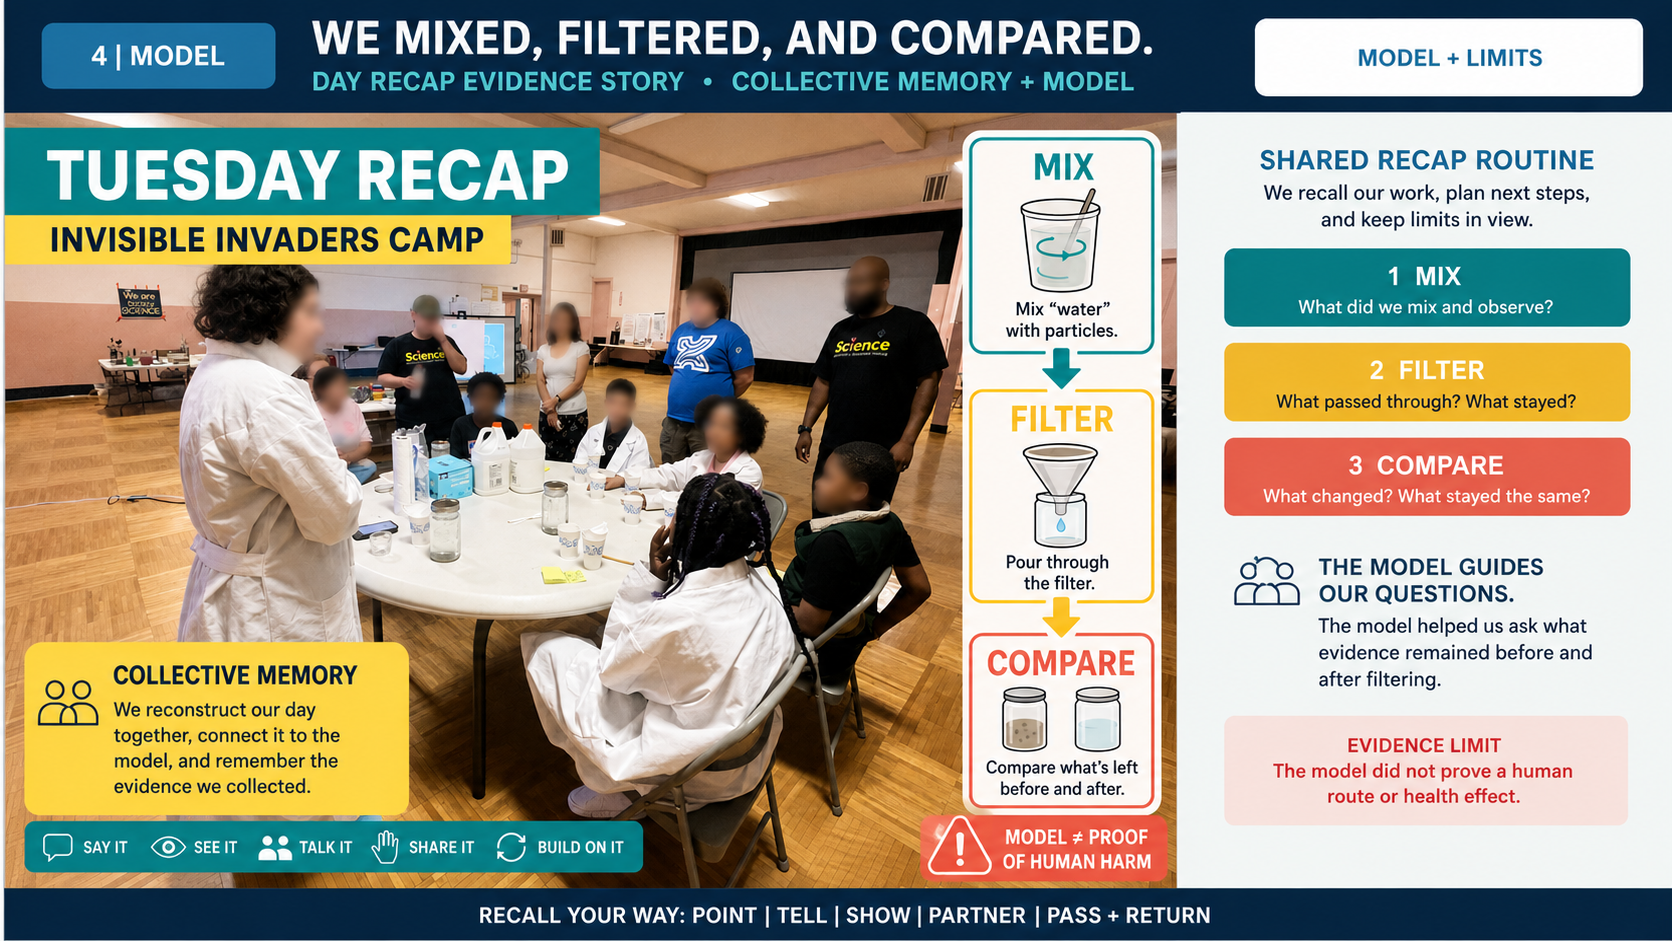
\includegraphics[
  width=0.85\textwidth,
  keepaspectratio
]{assets/artifact-previews/day-recap-day3-example.png}

% \vspace{0.015in}
\parbox{0.94\textwidth}{\centering
\textbf{\color{DeepNavy}Public-safe Day 3 recap example.}
The recap reconstructs a shared investigation through \textit{mix, filter, and compare}, reconnects the activity to the scientific model, preserves an explicit evidence limit, and keeps multiple recall routes available. The same record supports student memory, partner conversation, family communication, and planning for what should happen next.}

% \vspace{0.04in}
\makebox[\textwidth][c]{%
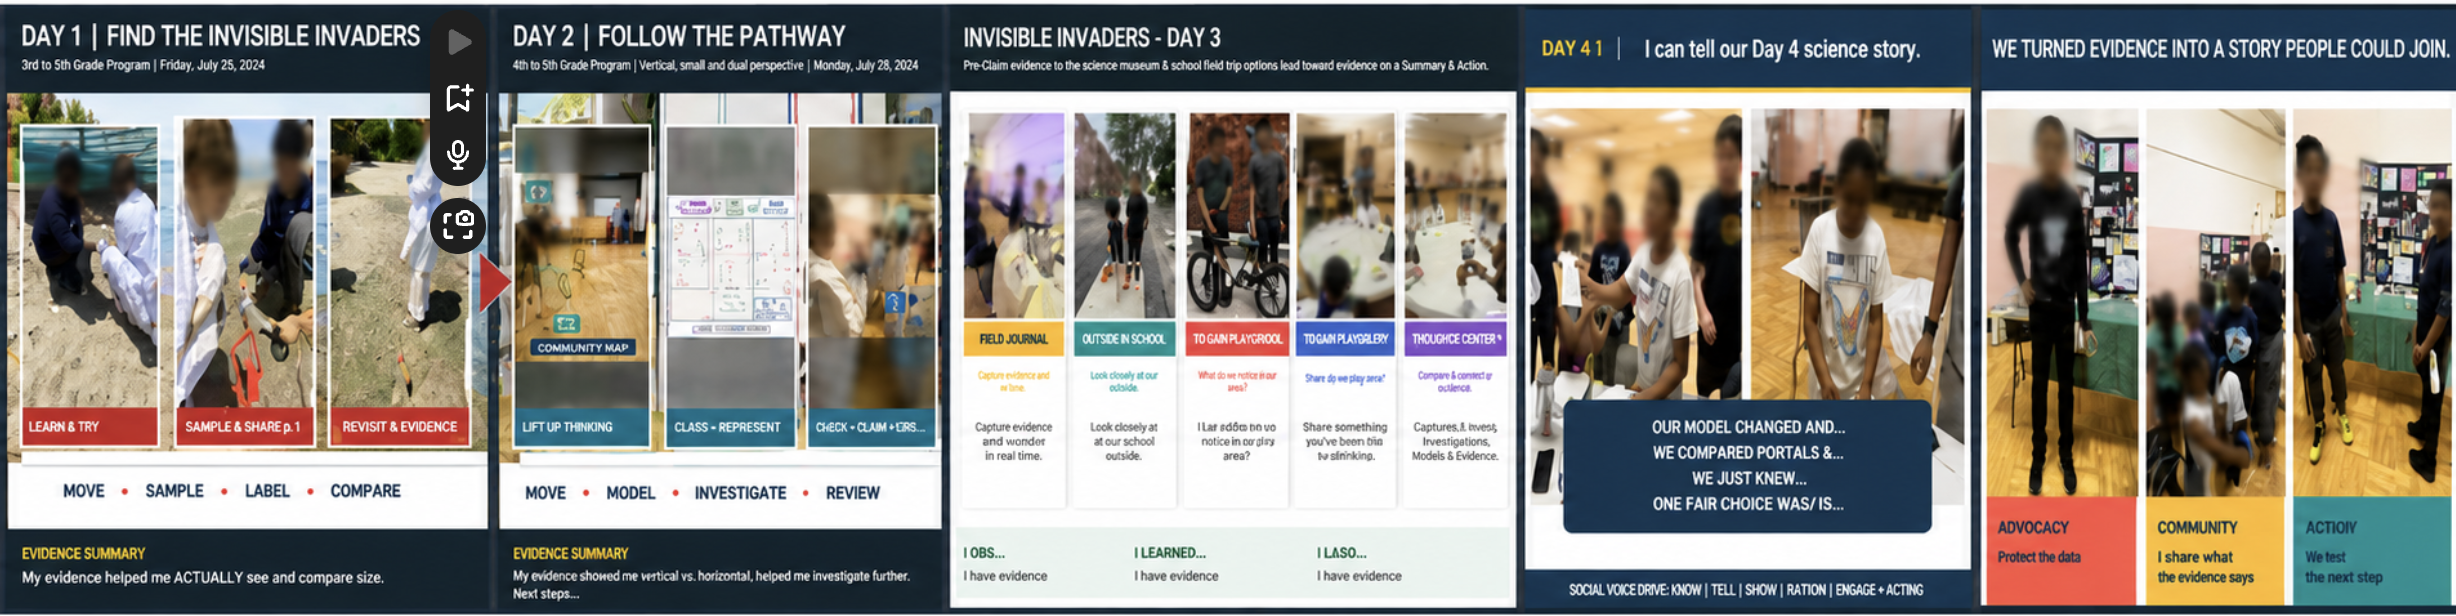
\includegraphics[
  width=1.0\textwidth,
  trim=0 100 0 100,
  clip
]{assets/artifact-previews/five-day-recap-strip.png}%
}
% \vspace{0.01in}
\parbox{0.94\textwidth}{\centering\textbf{Days 1--5 archive:}
locate the problem; collect and compare evidence; revise the model; examine living systems; and carry evidence into youth-led community action.}

\end{center}

\newpage
% \small

\toolsection{Build the Recap Before Planning Tomorrow}
\begin{spacing}{1.0}
\begin{enumerate}
  \item \textbf{Inventory what actually happened.} Record every activity, including what changed order, shortened, moved, expanded, or did not happen.
  \item \textbf{Triangulate the evidence.} Use artifacts, photographs, video/transcript records, student memos, measurements, and instructor notes according to what each source can actually establish.
  \item \textbf{Preserve youth meaning.} Record direct words, questions, choices, dislikes, model revisions, and contributions; do not infer understanding, emotion, or motivation from appearance alone.
  \item \textbf{Rebuild the shared storyline.} Show what the group did, what evidence changed the explanation, what remained uncertain, and what question should continue.
  \item \textbf{Keep communication and re-entry visible.} Preserve routes such as point, tell, show, partner, pass, and return, along with role changes, movement, sensory boundaries, and later re-entry.
  \item \textbf{Close the loop.} Use the reviewed recap to decide what to keep, change, stop, or investigate next, then circulate only the version appropriate for each approved audience.
\end{enumerate}
\end{spacing}

\toolsection{One Story, Four Feedback Loops}

\renewcommand{\arraystretch}{1.08}
\setlength{\tabcolsep}{4pt}

\begin{tabularx}{\textwidth}{
>{\bfseries\RaggedRight\arraybackslash}p{0.70in}
>{\RaggedRight\arraybackslash}p{2.98in}
>{\RaggedRight\arraybackslash}X}

\rowcolor{MidTeal}
\color{white}Audience &
\color{white}What the Recap Returns &
\color{white}What It Can Change \\

Youth &
A visible memory of the activities, their work, model changes, choices, and questions &
Correction, ownership, re-entry, reflection, and the next investigation \\

\rowcolor{SoftGray}
Teaching team &
One reviewed evidence story instead of isolated impressions or behavior labels &
Pacing, materials, questions, roles, supports, participation routes, and what stops/continues \\

Program partners &
Traceable claims, participation routes, plan decisions, revisions, and evidence limits &
Institutional understanding, resource decisions, and accountability for adult design \\

\rowcolor{SoftGray}
Families &
Concrete account of what youth did, shared, asked, learned, disliked, or wanted &
Family conversation, continuity across settings, and knowledge that can return to teachers\\

\end{tabularx}

\toolsection{Evidence That Changed the Story \& Puzzle Plan and EQUITAS in Practice}

The recaps changed how camp events were interpreted. Day 2 records the racket game as a movement reset and relationship route. Day 3 keeps ``point, tell, show, partner, pass + return'' available across the recap so remembering the day does not depend on one communication mode. The later youth retrospective asks for less rushing, more investigation time, more physical activity, a non-fish route to the same scientific idea, and numbered showcase stations. The evidence therefore changes the shared story and the design of what should happen next \citep{campEvidence2026}. The Puzzle Plan brings student voice together with artifacts, context, scientific evidence, and adult decisions. EQUITAS asks whose words enter the recap, who appears only as a body, and who gets to correct the institutional story. A recap becomes access-to-agency only when youth work can alter the record, interpretation, lesson, understanding, or what families receive.

\reflectionbox{\textbf{Artifact proof:} Five reviewed recap decks for Days 1--5 collectively preserve activities, youth contributions, communication routes, evidence limits, model revisions, and next questions. Day 6 has a clean retrospective transcript. Day 5 has photographs and a same-session transcript; its recap explicitly limits what photographs can establish \citep{campEvidence2026}.}

\adaptationbox{A recap can still privilege the most verbal, photographed, or adult-approved account. Invite correction through speech, AAC, writing, drawing, pointing, shared visuals, home language, partner support, or private review. Preserve disagreement, refusal, uncertainty, and ``not yet.''}

% \sourcebox{\scriptsize Camp recap archive \citep{campEvidence2026}; communication and behavior \citep{peckhamhardin2015behavior}.}

\normalsize
\resourceheading{8}{Low-Tech AAC Backup \& Vocabulary Starter}{AAC continuity and multimodal communication\par}{Communicators, families, teachers, speech-language pathologists \& support staff}{Module 3 multimodal system, AAC review, and EDU486 sensory feedback}

\vspace{-0.5cm}
\toolsection{What This Resource Is}

A shared record can preserve meaning only if the communicator can still express it when the primary route is unavailable. A low-tech backup is a printed or durable communication display that preserves access when a speech-generating device is charging, unavailable, difficult to position, unsafe near materials, or simply not preferred in that moment. It is not a lesser system or a test a learner must pass before ``earning'' technology. Multimodal AAC combines aided and unaided methods, and the available route should change with the communicator's needs, preferences, and context without reducing the range of messages they can express \citep{ashaAAC,mirenda2015aids}. The starter below organizes vocabulary by communicative function rather than by adult task. The communicator and speech-language pathologist should determine representation, language, field size, layout, symbol system, color, spacing, contrast, and access method. When useful for motor planning, important vocabulary should remain in predictable locations across the primary and backup systems.

\toolsection{Core, Context, and Repair Starter}

\renewcommand{\arraystretch}{1.00}
\setlength{\tabcolsep}{3pt}

\begin{tabularx}{\textwidth}{|>{\centering\arraybackslash}p{0.60in}|>{\centering\arraybackslash}p{0.70in}|>{\centering\arraybackslash}p{0.70in}|>{\centering\arraybackslash}X|>{\centering\arraybackslash}X|>{\centering\arraybackslash}X|}
\hline
\rowcolor{SoftBlue}
\textbf{I} & \textbf{you} & \textbf{it} & \textbf{want} & \textbf{not} & \textbf{more} \\
\hline

\rowcolor{SoftGreen}
\textbf{go} & \textbf{stop} & \textbf{help} & \textbf{look} & \textbf{think} & \textbf{like} \\
\hline

\rowcolor{SoftGold}
\textbf{different} & \textbf{same} & \textbf{tell} & \textbf{why} & \textbf{where} & \textbf{when} \\
\hline

\rowcolor{SoftRose}
\textbf{wait} & \textbf{not that} & \textbf{show me} & \textbf{say another way} & \textbf{you misunderstood} & \textbf{something else} \\
\hline
\end{tabularx}

\vspace{0.08in}

Keep the core stable and add a small, changeable context strip instead of crowding the board. For an evidence-to-action science routine, possible vocabulary includes:

\begin{center}
\colorbox{SoftGray}{\parbox{0.94\textwidth}{\centering\small
\textbf{evidence \quad compare \quad count \quad model \quad revise \quad sample \quad tire \quad litter \quad microscope}\par
\vspace{0.03in}
\textbf{smell \quad texture \quad observe only \quad no fish \quad different material \quad ready later \quad policy \quad showcase}
}}
\end{center}

\toolsection{Build and Use Checklist}

\begin{enumerate}
  \item \textbf{Start with the communicator.} Confirm current modes, languages, vocabulary priorities, visual and literacy access, and whether a printed board is wanted.
  \item \textbf{Match the access route.} Use direct pointing, eye pointing, partner-assisted scanning, a switch-compatible sequence, or another reliable method.
  \item \textbf{Protect the full message range.} Include refusal, sensory and pain messages, questions, comments, humor, academic language, repair, and requests for more time---not only requests for objects.
  \item \textbf{Place backups where communication happens.} Keep copies at the desk, in activity materials, during transport, at home, or in an emergency kit as appropriate.
  \item \textbf{Model without demanding imitation.} Partners may point to words while speaking, then wait and accept the communicator's response through any reliable mode.
  \item \textbf{Audit the system.} Record missing vocabulary, access failures, damaged or unavailable boards, and whether communicated messages actually changed what happened.
\end{enumerate}

\toolsection{Continuity Plan}
\begin{center}
{\scriptsize\bfseries\color{DeepNavy}
Communication Continuity: Same Message Range, Different Route}
\begin{tikzpicture}[
  route/.style={
    draw=DeepNavy,
    rounded corners=2pt,
    minimum width=1.2in,
    minimum height=0.1in,
    align=center,
    font=\tiny,
    inner sep=2pt
  },
  link/.style={
    <->,
    >=Latex,
    line width=0.35pt,
    draw=PrimaryRed
  }
]

\node[route, fill=SoftBlue] (device)
  {\textbf{HIGH-TECH AAC}\\ speech-generating system};

\node[route, fill=SoftGreen, right=0.34in of device] (paper)
  {\textbf{PRINTED BACKUP} stable vocabulary locations};

\node[route, fill=SoftGold, right=0.34in of paper] (other)
  {\textbf{OTHER RELIABLE MODES}\\ gesture, writing, visual, object};

\draw[link] (device) -- (paper);
\draw[link] (paper) -- (other);

\node[
  draw=MidTeal,
  fill=SoftGreen,
  rounded corners=2pt,
  below=0.11in of paper,
  text width=5.90in,
  align=center,
  font=\tiny,
  inner sep=1pt
]
{\textbf{The message range travels too:}
stop \quad help \quad different \quad question \quad repair \quad more time \quad sensory boundary.};
\end{tikzpicture}

\vspace{-0.2cm}
{\tiny \par The route can change without shrinking agency; continuity preserves the communicator's ability to participate, revise, refuse, teach, and influence.}
\end{center}

Name who prints and updates the board, who checks availability, where backups live, and how partners will respond when the primary system is unavailable. Important vocabulary and predictable locations should travel across systems when useful, but the learner should never be forced onto the paper board when gesture, writing, an object, a shared visual, or another route communicates the message more clearly. Continuity means preserving the communicator's message and influence across tools, people, settings, and time. Puzzle Plan tracks if the meaning survives the route change; EQUITAS asks if the communicator still controls refusal, correction, and audience. Implementation reliability remains a system responsibility \citep{norrie2021context}.

\begin{center}

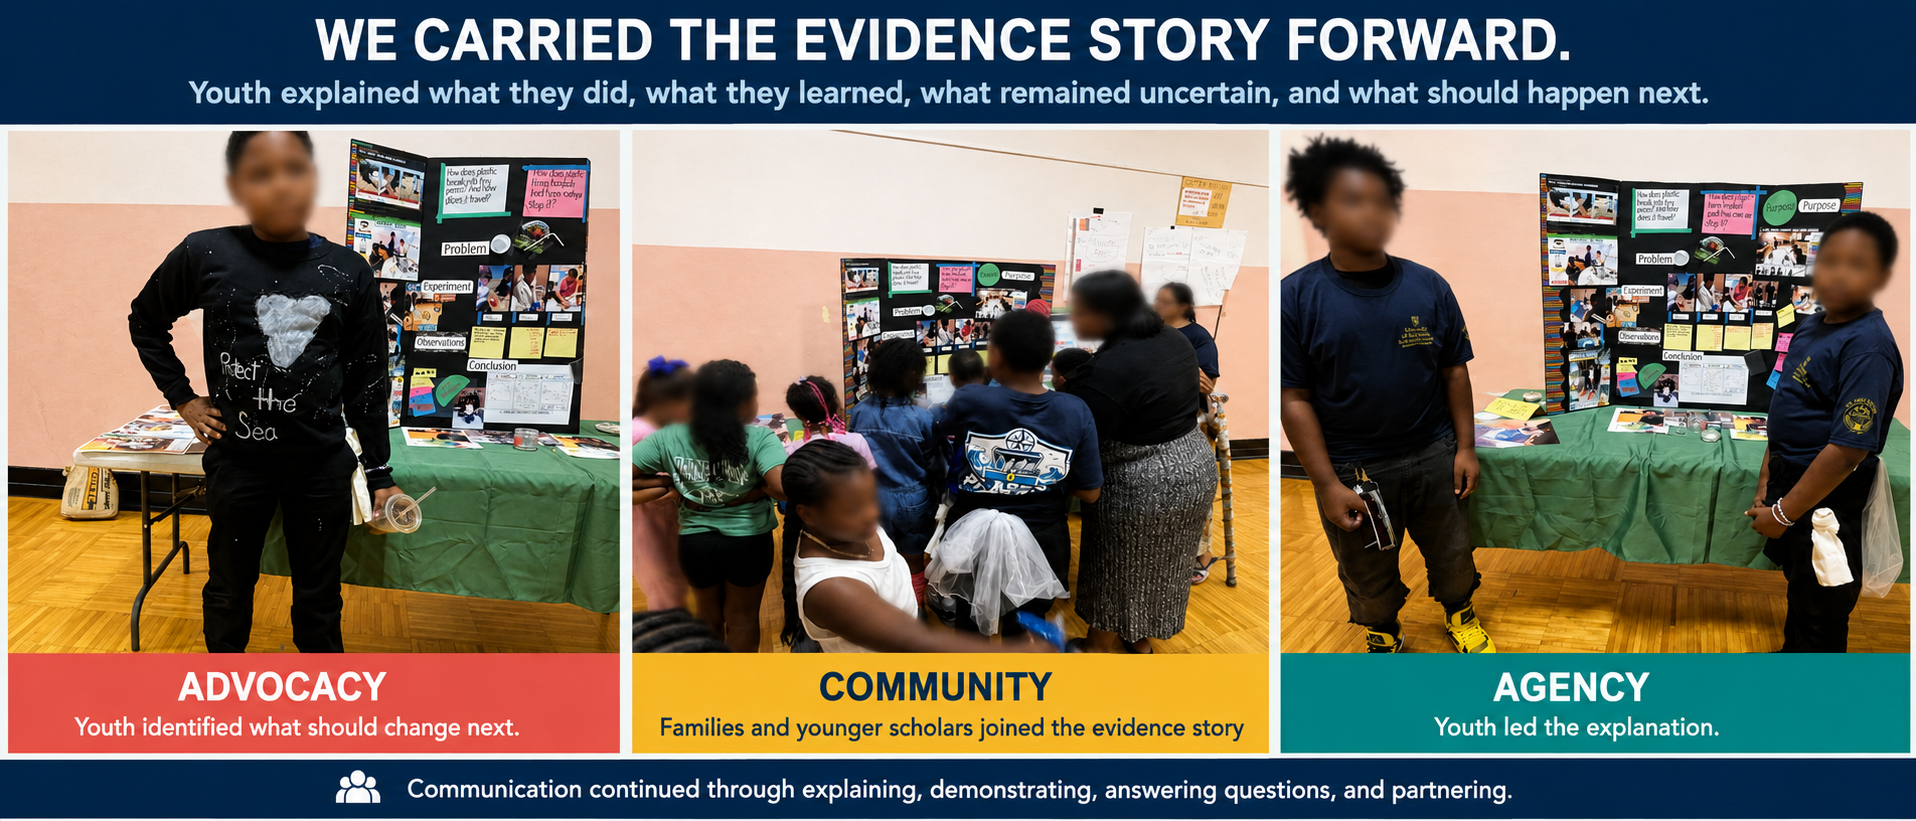
\includegraphics[
  width=0.8\textwidth,
  keepaspectratio
]{assets/artifact-previews/youth_carry_the_evidence_forward.png}

\parbox{1.0\textwidth}{\centering\textbf{\color{DeepNavy}Communication Continuity Beyond the Device.}
Youth carried the week's evidence into a new audience of families, visitors, and younger scholars. They explained, demonstrated, pointed, answered questions, partnered with others, and used the shared evidence display to reconstruct what they had done, what remained uncertain, and what they believed should happen next. Communication continued because the message could travel through different people and modes \citep{campEvidence2026}.}
\end{center}

\reflectionbox{\textbf{Practice artifact --- vocabulary from youth feedback:} Camp feedback showed why a backup system must include more than academic vocabulary. Youth identified smell and texture as barriers in the fish activity and proposed changes for future participation. A mask was one suggestion, but equipment does not equal consent. The context strip therefore includes \textit{smell, texture, observe only, no fish, different material,} and \textit{ready later} alongside science words. Those messages became design evidence: youth could communicate what should continue, what should change, and what future participants might need. A backup therefore preserves not only participation in the present activity, but the learner's ability to influence what happens next \citep{campEvidence2026}.}

\adaptationbox{A dense grid may be inaccessible because of vision, motor, literacy, language, sensory, or attention needs. Reduce field size, increase spacing or contrast, use photographs or objects, add partner-assisted scanning, or create layered displays while preserving robust message functions. Do not change symbol locations casually. Trial revisions with the communicator, and treat rejection of the board as information about the system rather than noncompliance. Continuity succeeds when the learner's meaning remains available even when the route, partner, activity, or audience changes.}

\sourcebox{ASHA AAC overview \citep{ashaAAC}; multimodal AAC design \citep{mirenda2015aids}; implementation context \citep{norrie2021context}; de-identified camp feedback/evidence.}
\resourceheading{9}{Full-Week Personalized Family Recap}{Family communication, student authorship, and learning continuity\par}{Students, families, teachers, and support teams}{Module 3 Daily Communication Logs critique and completed EDU486 day-by-day recap books}

\vspace{-0.5cm}
\toolsection{The Existing Camp Artifact}

This resource grew directly from how I wanted families to see the week: as a record of what they did, noticed, questioned, contributed, and helped shape. For each of our two assigned youth, we created a personalized full-week recap book. One completed book contains five landscape pages for Days 1--5, and each attended day has its own page built around an action image, a transcript-grounded contribution, a concise science story, and five activity memories connecting what the learner did to why it mattered \citep{campEvidence2026}. The science moves (observing, modeling, testing, asking, and acting) help make participation visible with dignity. Each page also includes an evidence boundary so that what we observed remains separate from what we interpreted or could not confirm. This gives learners and families something concrete they can point to, retell, question, or correct together. Personalized email drafts were also prepared to introduce the books and invite families to review them with the learner.

\toolsection{Per Day and Per Activity: The Completed Page}
\begin{center}

\restrictedartifact
  {assets/artifact-previews/weekly-recap-day3-example.png}
  {0.85\textwidth}

\parbox{1.0\textwidth}{\centering
\textbf{\color{DeepNavy}Personalized Day 3 Science Story.}

The completed page centers the learner as an investigator, preserves a grounded contribution, and reconstructs the day through activity memories. Each card connects action to thinking while the evidence boundary states what the camp record establishes. It functions as a learning record and a memory support: the learner can point to an activity, retell in their own way, and revisit how their thinking developed.
}

\end{center}

\newpage
\small

\toolsection{From Rating Log to Family Learning Story}

The EDE448 Daily Communication Logs packet offers useful structures for home--school communication, but several examples foreground good/fair/poor days, warnings, sitting, compliance, or adult initials \citep{dailylogs2009}. The completed camp recap books demonstrate a different communication architecture: they organize the record around what the learner did, communicated, questioned, contributed, and was still working to understand.

\renewcommand{\arraystretch}{1.00}
\setlength{\tabcolsep}{3pt}

\begin{tabularx}{\textwidth}{
>{\bfseries\RaggedRight\arraybackslash}p{1.19in}
>{\RaggedRight\arraybackslash}p{2.70in}
>{\RaggedRight\arraybackslash}X}

\rowcolor{MidTeal}
\color{white}Adult-Centered Pattern &
\color{white}Recap-Book Shift &
\color{white}Support Value \\

Good/fair/poor day &
Observable activity, contribution, learner words or action, and an evidence limit &
Context replaces moral rating \\

\rowcolor{SoftGray}
Warnings, sitting, compliance &
Choices, questions, refusals, sensory boundaries, roles, movement, and re-entry &
The learner appears as a communicator and participant, not a management problem \\

One summary box &
One page per attended day and five activity cards within each page &
Differences across activities, roles, and access needs remain visible \\

\rowcolor{SoftGray}
Adult initials as authorship &
Student words, artifacts, documented actions, learner review, and family invitation &
Authorship and correction are distributed rather than owned by one adult \\

Finished-sounding claim &
``Still to test,'' ``not confirmed,'' or another precise evidence boundary &
Uncertainty remains visible, honest, and useful \\

\rowcolor{SoftGray}
Required family return &
Optional response through a chosen mode, time, or not at all &
Family participation is invited without treating silence as lack of care \\

\end{tabularx}

\toolsection{Ready-to-Use Record / Student-Centered Entry (Reconstructed Example)}

\renewcommand{\arraystretch}{1.12}
\setlength{\tabcolsep}{4pt}
\begin{tabularx}{\textwidth}{>{\bfseries\RaggedRight\arraybackslash}p{1.55in} >{\RaggedRight\arraybackslash}X}
\rowcolor{MidTeal}
\color{white}Entry Field & \color{white}De-identified Camp-to-Home Example \\
Day and attendance & Day 3 attended (Invisible Invaders weekly recap sequence; five activity cards reviewed) \\
\rowcolor{SoftGray}
Observable participation & Joined sampling and evidence-talk tasks; pointed to sample locations, verbally compared findings with a partner, and used ``pass + return'' before rejoining group reporting \\
Access supports used & Visual activity sequence, point/tell/show/partner/pass + return routes, processing time, movement re-entry option, and choice to observe-only for high-smell materials \\
\rowcolor{SoftGray}
Concise camp-to-home update & ``Today your child helped compare sample evidence, named one hands-on part they liked, and returned to the group after a short break. The team marked what is confirmed vs. still to test in the recap.'' \\
Optional family-return area (blank by design) & \textbf{Optional reply only if helpful:} Home connection noticed: \underline{\hspace{1.85in}}\\[0.05in]
& Preferred support for next session: \underline{\hspace{1.5in}}\\[0.05in]
& Best return mode (text/email/paper/audio/none): \underline{\hspace{1.25in}} \\
\end{tabularx}

\vspace{0.04in}
\noindent\footnotesize\textit{Evidence boundary: Day attendance structure, activity-sequence reporting, access routes, and prepared family-invite workflow are documented in the camp archive; the blank family-return prompts above are a proposed reusable format and are not a recovered parent reply} \citep{campEvidence2026}.
\normalsize

\toolsection{Prepare, Review, and Deliver}

\begin{enumerate}
  \item \textbf{Verify identity and access.} Confirm attendance, name, pronouns, languages, intended readers, and permissions.
  \item \textbf{Assemble the evidence.} Gather student memos, artifacts, recap materials, images, and the activity sequence.
  \item \textbf{Separate evidence from interpretation.} Mark exact words, documented actions, team evidence, interpretations, and unknowns before designing the page.
  \item \textbf{Return control to the learner.} When possible, let the learner select, edit, translate, restrict, replace, or withhold parts of the outgoing story.
  \item \textbf{Review the complete record.} Check every attended day, all activity cards, attribution, accessibility, privacy, and evidence limits before export.
  \item \textbf{Deliver without overclaiming.} Use an approved communication channel, document receipt when available, and invite a low-burden response. Without evidence of delivery, say \textit{prepared for family delivery}, not \textit{sent}.
\end{enumerate}

\toolsection{Puzzle Plan and EQUITAS in Practice}

The Puzzle Plan carries the student memo, daily souvenir, team recap, activity evidence, and week-long storyline forward without collapsing them into one adult judgment. Each source contributes a different piece of the learner's experience. EQUITAS asks who controls the family narrative, whose activities or communication routes are missing, whether interpretation is clearly labeled, whether uncertainty remains visible, and whether the family has an accessible way to return knowledge to the team. Family knowledge is part of the evidence system \citep{zacarian2015community}.

\reflectionbox{\textbf{Artifact and delivery proof:} The private production bundle contains two final personalized recap PDFs, plus review renders, source records, image manifests, and two personalized email drafts \citep{campEvidence2026}.}

\adaptationbox{Family communication can become surveillance or burden. Collect only information that supports learning, communication, access, or continuity; follow privacy policy; use approved channels; and honor preferences for translation, audio, paper, event-triggered updates, weekly summaries, no photographs, no specific message, or no formal log at all.}

% \sourcebox{\scriptsize Daily Communication Logs \citep{dailylogs2009}; family recap archive \citep{campEvidence2026}; classroom-community partnership \citep{zacarian2015community}.}

\normalsize
\resourceheading{10}{Flexible Peer Roles and Participation Routes}{Social interaction, group work \& executive-function access\par}{Teachers, students, families, and activity leaders}{Kit for Kids lesson design, EDU486 camp \& Module 3 communication planning}

\vspace{-0.5cm}
\toolsection{What This Resource Is}

The same principle of distributed knowledge applies inside group work: belonging should not depend on one pace, posture, communication mode, sensory tolerance, or public role. This tool combines the Kit for Kids peer actions (\textit{invite, wait, ask, and respect}) with visible, changeable roles and explicit permission to observe, pass, pause, and return \citep{oar2026kit,oar2026tips}. The goal is to make the intellectual and social work of the group accessible while preserving choice, challenge, and meaningful contribution. Peer interaction becomes a rich communication context when students can initiate, direct, disagree, ask questions, repair misunderstandings, revise ideas, and influence shared work \citep{downing2015classroom}. Group systems therefore need to teach peers how to support without taking over while also requiring adults to redesign barriers such as noise, rushed timing, unclear roles, competition for materials, or an expectation that everyone respond aloud. Camp practice reinforced the same principle. Participation included measuring, observing, recording, speaking, partnering, stepping back, and returning rather than treating continuous visible engagement as the only acceptable route \citep{campEvidence2026}. A flexible role system makes those routes explicit before a learner has to struggle to create one.

\toolsection{Flexible Role Menu}

% \small
\renewcommand{\arraystretch}{1.0}
\setlength{\tabcolsep}{3pt}

\begin{longtable}{
>{\bfseries\RaggedRight\arraybackslash}p{0.90in}
>{\RaggedRight\arraybackslash}p{2.40in}
>{\RaggedRight\arraybackslash}p{3.60in}}

\tableheaderthree{Role}{Possible Contribution}{Access Routes and Safeguards}

Starter/\newline modeler &
Begin one step, demonstrate a possible move, or make an idea visible &
Use materials, a photograph, gesture, drawing, code, AAC, or partner support; another student may begin \\

\rowcolor{SoftGray}
Evidence finder &
Notice, collect, compare, locate, or point to information &
Use direct contact or non-contact observation, camera, magnifier, label, pointer, or partner handling; sensory contact is never required \\

Recorder/\newline mapper &
Preserve ideas, changes, questions, evidence, or group decisions &
Write, type, draw, photograph, arrange symbols, dictate, or direct a partner without requiring handwriting or continuous note taking \\

\rowcolor{SoftGray}
Connector/\newline questioner &
Ask how ideas fit, request clarification, invite another perspective, or identify what is still unknown &
Use speech, a prepared card, AAC, private note, pointing, writing, or a partner-read question \\

Materials/\newline access lead &
Organize tools and help notice whether everyone reaches the work &
Ask before moving another person's materials, seat, device, or communication system; the role supports access rather than controlling peers \\

\rowcolor{SoftGray}
Reviser/\newline debugger &
Test an idea, disagree, locate a problem, or propose another route &
``Not that,'' ``try again,'' ``I disagree,'' and ``something else'' remain valued contributions \\

Presenter/\newline demonstrator &
Share or demonstrate the group's learning for another audience &
Speak, show, point, play media, hold proof, use AAC, co-present, answer privately, or present another way \\

\rowcolor{SoftGray}
Observer/\newline returner &
Watch first, track the process, pause participation, and enter later through a named step &
The role includes a visible re-entry route and cannot become a holding place that excludes the learner from substantive intellectual work \\

\end{longtable}

\normalsize

\toolsection{Group Start Script}

Display shared goals, known materials, approximate time, and the role menu before the group starts. Say:

\begin{quote}
\textit{Choose a way to begin. You may take one role, combine roles, ask for a different one, observe first, or pass and return. Ask before helping. Wait for a response. Keep communication tools with their owner. A strong group changes its plan when someone identifies an access barrier.}
\end{quote}

Make useful group language available before students need it: \textit{my turn, your turn, wait, help, show me, not yet, stop, different role, I disagree, I have an idea, you misunderstood,} and \textit{I am ready to return}. These messages may be spoken, written, pointed to, signed, selected through AAC, or communicated through another reliable route. Use a visible turn sequence if it supports access; do not require students to contribute in only one way.

% \small
\toolsection{When Group Work Breaks Down}

\renewcommand{\arraystretch}{1.0}
\setlength{\tabcolsep}{3pt}

\begin{tabularx}{\textwidth}{
>{\RaggedRight\arraybackslash}p{1.35in}
>{\RaggedRight\arraybackslash}p{2.25in}
>{\RaggedRight\arraybackslash}X}

\rowcolor{PrimaryRed}
\color{white}What Adults Notice &
\color{white}Possible Barrier to Investigate &
\color{white}Support Match \\

One student controls tools or talk &
Roles or turn-taking are unclear; helping has become takeover &
Return tool ownership, offer role and turn choices, teach ask-and-wait \& create an independent route \\

\rowcolor{SoftGray}
Student withdraws, pauses, or leaves &
Noise, crowding, uncertainty, processing demand, conflict, fatigue, pain, or an unwanted role &
Offer space, a lower-load route, a private check-in, another group size or role, and a clear step for returning \\

Group rushes one member &
Speed is treated as competence and wait time is not protected &
Remove race language, offer flexible timing, allow asynchronous contribution \& model real waiting \\

\rowcolor{SoftGray}
An idea is ignored &
Communication mode, status, or group dynamics determine whose evidence counts &
Record proposals visibly, confirm meaning, provide private or anonymous routes, and require decisions to reference evidence, not popularity \\

Peer ``helps'' without consent &
Assistance has been praised without boundaries or the learner's control has been displaced &
Ask first, offer choices, accept ``no,'' return control of the task or tool, and repair the interaction when needed \\

\end{tabularx}

\normalsize
\toolsection{Review With Students}

Review the group process with the same attention given to the final product. Ask which roles were meaningful, whose ideas changed the work, whether anyone had to perform a preferred style to participate, where communication became difficult, and what adults should redesign. Record contribution through multiple forms. Constructing competence means designing environments that expect meaningful contribution while supplying the access necessary to make it possible \citep{jorgensen2018competence}. Puzzle Plan records whose contribution changed the product; EQUITAS asks how the role structure distributes influence and supports inclusion.

\reflectionbox{\textbf{Practice artifact, camp role trail:} Camp participation often changed form without losing intellectual value. During measurement, one youth self-selected the role of ``commentator'' and watched for visible litter. Identity Beads recognized contributions such as designer, environmental advocate, altruist, brave scientist, motivator, investigator, inventor, storyteller, or another youth-authored identity without ranking one above another. Policy work introduced mayor, parks, tourism, restaurant, and environmental-scientist perspectives while preserving vote. At the final showcase, youth could demonstrate, point, answer, ask a visitor a question, hold evidence, or partner with another speaker. Across these activities, roles carried real intellectual and social work and remained changeable.}

\adaptationbox{Peer structures cannot compensate for inaccessible instruction. Adults still have to address noise, pace, material layout, language demands, conflict, social status, and whose communication is recognized. Do not create a permanent helper, spokesperson, or observer role for a learner. Revisit roles across activities, protect private and bilingual communication, and treat refusal, withdrawal, or a request for individual work as information about access. A participation route is successful when it preserves both belonging and influence.}

% \sourcebox{\scriptsize OAR peer-education resources \citep{oar2026kit,oar2026tips}; rich communicative environments \citep{downing2015classroom}; communicative competence \citep{jorgensen2018competence}; de-identified camp evidence \citep{campEvidence2026}.}

\clearpage
\section*{Portfolio-Wide Reflection and Revision Commitments}
\addcontentsline{toc}{section}{Portfolio-Wide Reflection and Revision Commitments}

\begingroup
\small
\setstretch{1.0}
\setlength{\parskip}{0.045in}

\toolsection{From Teaching Placement to Course Practice}

Across this portfolio, my central learning is that inclusion is created when sensory conditions, communication routes, peer norms, roles, and adult responses allow learners to understand, contribute, question, refuse, repair, return, and influence. My teaching placement at Pine Brook made this concrete. Competence in technology-rich lessons could be obscured by rapid directions, noise, crowded materials, unclear roles, peer pacing, or removal of a familiar tool. On one occasion, a learner joined a blocks activity after adults removed the either--or condition requiring the learner to give up a familiar laptop. Changing the condition revealed participation the original design had concealed. The sensory walk, Kit for Kids lesson, and PTR inquiry pushed me to examine conditions before judging behavior, separate observation from inference, teach peers to support without taking over, and redesign barriers before demanding tolerance \citep{guggenheimSensory,michigan2025sensory,oar2026kit,dunlap2019ptr}.

EDE448 extended that lesson across communication and positive support. Sensory access should be proactive, peer culture is part of the support environment, AAC is multimodal, and competence develops through opportunity, responsive partners, meaningful roles, and consequential messages \citep{ashaAAC,downing2015classroom,jorgensen2018competence,peckhamhardin2015behavior}. EDU486 camp tested those principles across real activities. Youth could point, tell, show, write, partner, pass, return, change roles, and use movement as a reset while doing rigorous environmental-science work \citep{campEvidence2026}. Flexible routes separated the learning goal from one required pace, posture, sensory tolerance, communication mode, or performance style.

\toolsection{What Puzzle Plan and EQUITAS Produced}

The \textsc{Puzzle Plan} turned these lessons into a connected evidence-to-design cycle. It places lived experience, student words, observable action, work products, scientific records, context, family knowledge, and adult decisions beside one another so no single source becomes the whole story. The camp artifacts illustrate that cycle across time: a video memo preserves an immediate account; a daily souvenir reconstructs a contribution; a day recap connects activities, evidence limits, and next questions; and a full-week recap carries that learning story across settings. At the final showcase, youth moved from participating in investigations to explaining evidence, uncertainty, and possible solutions to families, visitors, and younger scholars \citep{campEvidence2026}. The ten portfolio resources translate the same logic into sensory redesign, peer instruction, PTR, student voice, AAC, family partnership, evidence stories, and flexible roles. Across them, evidence matters because it can change a teaching decision.

\textsc{EQUITAS}, the equity-centered heart of the Puzzle Plan, asks: \textit{Whose knowledge enters the record? Whose contribution disappears? What context is missing? Who controls the interpretation? Who can disagree, refuse, revise, or correct the story?} Those questions produced safeguards throughout the portfolio: multiple communication routes, wait time, pass-and-return options, consent, bilingual and low-tech access, changeable roles, and explicit evidence boundaries. Most notably, EQUITAS requires evidence that communication has consequences. A learner's message should be able to change materials, pacing, roles, access, questions, conditions, or an adult decision. If support reduces visible disruption while also reducing communication, trust, dignity, agency, or belonging, quieter behavior cannot be treated as success.

\toolsection{Families, Community, and Revision Commitments}

This work widened my understanding of where inclusion happens and who participates in producing it. A family-facing learning story should give the learner meaningful control over what travels home while creating an accessible route for families to contribute language, context, priorities, questions, and interpretations. Family knowledge belongs inside the evidence system \citep{zacarian2015community}. Responsibility is similarly distributed across the learning community: peers practice \textit{invite, wait, ask, and respect}; educators design communication and sensory access; families contribute knowledge that may not be visible at school; and collaborators share responsibility for implementation. Community-facing science, policy roles, and choices can carry learning beyond the classroom while preserving dignity. Inclusion therefore redistributes responsibility for access, interpretation, and participation across the learning community.

My revision commitment is to co-design these tools across languages and communication modes; track adult implementation and whether learner messages produce change; provide accessible, translated, low-tech, no-photo, no-message, and private routes; invite family and community knowledge without unnecessary burden; and distinguish what was \textit{planned, prepared, delivered, received, observed, interpreted,} and \textit{learned}. The evidence boundaries developed throughout this portfolio will remain central. The teacher's work is not to complete the puzzle for another person. \textsc{Puzzle Plan} keeps the pieces connected; \textsc{EQUITAS} asks who has power over their meaning. Together, they move communication from access toward agency: learners gain more ways to author, question, revise, and shape what happens next.
\endgroup

\clearpage
\bibliography{references}

\end{document}